%% The "\appendix" call has already been made in the declaration
%% of the "appendices" environment (see thesis.tex).
\chapter{Pointless extras}
\label{app:Pointless}

\chapterquote{%
Le savant n'\'etudie pas la nature parce que cela est utile; \\
\indent il l'\'etudie parce qu'il y prend plaisir, \\
\indent et il y prend plaisir parce qu'elle est belle.}%
{Henri Poincar\'e, 1854--1912}

Appendixes (or should that be ``appendices''?) make you look really clever, 'cos
it's like you had more clever stuff to say than could be fitted into the main
bit of your thesis. Yeah. So everyone should have at least three of them\dots

\section{Anomalous Gauge Coupling Quartic Vertices Of Relevance in Vector Boson Scattering}
\label{sec:expansionalpha4alpha5}

The anomalous gauge couplings involving $\alpha_{4}$ and $\alpha_{5}$ arise in EFT through the addition of the following terms to the Lagrangian.

\begin{equation}
\text{Tr}(V^{\mu}V_{\nu})] \text{Tr}(V^{\nu}V_{\mu})] \text{ and } [\text{Tr}(V^{\mu}V_{\mu})]^{2} 
\end{equation}

Where $V_{\mu}$ is defined in the following way.

\begin{equation}
V_{\mu} = \Sigma(D_{\mu}\Sigma)^{\dagger}
\end{equation}
%V_{\mu} = ig\frac{\sigma^{i}}{2}W^{i}_{\mu} + i\frac{g'}{2}B_{\mu}

and $\Sigma$, the Higgs field matrix, is defined as. 

\begin{equation}
\Sigma = \text{exp}(-\frac{i}{v}\textbf{w})
\end{equation}

Where $\textbf{w} = w^{a} \sigma^{a}$.  $w^{a}$ are the ... and $\sigma^{a}$ are the Pauli spin matrices.  The covariant derivative of the Higgs field matrix is

\begin{equation}
D_{\mu}\Sigma = (\partial_{\mu} + \frac{ig}{2}W_{\mu} - \frac{ig'}{2}B_{\mu}\sigma^{3})\Sigma
\end{equation}

For clarity consider the unitarity gauge where $\textbf{w} = 0$, which implies $\Sigma = 1$.  In this gauge $V_{\mu}$ takes the following form.

\begin{equation*}
V_{\mu} = \frac{i}{2}(gW_{\mu}^{i}\sigma^{i} - g'B_{\mu}\sigma^{3}) = \frac{i}{2}
  \begin{pmatrix}
    gW_{\mu}^{3} - g'B_{\mu} & g(W_{\mu}^{1} - iW_{\mu}^{2}) \\
    g(W_{\mu}^{1} + iW_{\mu}^{2}) & -gW_{\mu}^{3} + g'B_{\mu}
  \end{pmatrix} \\
= \frac{i}{2}
  \begin{pmatrix}
    \sqrt{g^{2} + g'^{2}} Z_{\mu} & g\sqrt{2}W^{+}_{\mu} \\
    g\sqrt{2}W^{-}_{\mu} & \sqrt{g^{2} + g'^{2}} Z_{\mu}
  \end{pmatrix}
\end{equation*}

Where the relationship between the mass and gauge symmetry basis are as follows.

\begin{equation}
  W^{+}_{\mu} = \frac{1}{\sqrt{2}}(W^{1}_{\mu} - i W^{2}_{\mu}) \\
  W^{-}_{\mu} = \frac{1}{\sqrt{2}}(W^{1}_{\mu} + i W^{2}_{\mu}) \\
  Z_{\mu} = c_{w}W^{3}_{\mu} - s_{w}B_{\mu} \\
  A_{\mu} = s_{w}W^{3}_{\mu} + c_{w}B_{\mu}
\end{equation}

With $c_{w} = \frac{g}{\sqrt{g^{2} + g'^{2}}}$ and $s_{w} = \frac{g'}{\sqrt{g^{2} + g'^{2}}}$.  Consider the expansion of the terms to be incldued in the Lagrangian.

\begin{equation}
V^{\mu}V_{\nu} = \frac{-1}{4}
  \begin{pmatrix}
    \sqrt{g^{2} + g'^{2}} Z^{\mu} & g\sqrt{2}W^{+\mu} \\
    g\sqrt{2}W^{-\mu} & \sqrt{g^{2} + g'^{2}} Z^{\mu}
  \end{pmatrix}
  \begin{pmatrix}
    \sqrt{g^{2} + g'^{2}} Z_{\nu} & g\sqrt{2}W^{+}_{\nu} \\
    g\sqrt{2}W^{-}_{\nu} & \sqrt{g^{2} + g'^{2}} Z_{\nu}
  \end{pmatrix}
\end{equation}

\begin{equation}
  \text{Tr}[V^{\mu}V_{\nu}] = \frac{-1}{2} ((g^{2} + g'^{2})Z^{\mu}Z_{\nu} + g^{2}W^{+\mu}W^{-}_{\nu} + g^{2}W^{-\mu}W^{+}_{\nu}) 
\end{equation}

\begin{equation}
  \text{Tr}[V^{\mu}V_{\nu}]\text{Tr}[V_{\mu}V^{\nu}] = \frac{(g^{2} + g'^{2})^2}{4}(Z^{\mu}Z_{\mu})^{2} + g^{2}(g^{2} + g'^{2})(Z^{\mu}Z^{\nu}W^{-}_{\mu}W^{+}_{\nu}) \\
+ \frac{g^{4}}{2}(W^{-\mu}W^{+}_{\mu})^{2} + \frac{g^{4}}{2}(W^{-\mu}W^{+\nu}W^{-}_{\mu}W^{+}_{\nu})
\end{equation}

\begin{equation}
  \text{Tr}[V^{\mu}V_{\mu}]^{2} = \frac{(g^{2} + g'^{2})^2}{4}(Z^{\mu}Z_{\mu})^{2} + g^{2}(g^{2} + g'^{2})(Z^{\mu}Z^{\nu}W^{-}_{\mu}W^{+}_{\nu}) \\
+ g^{4}(W^{-\mu}W^{+}_{\mu})^{2}
\end{equation}

These two terms change the cross section for the vector boson scattering processes at CLIC that involve $ZZ \rightarrow ZZ$, $W^{+}W^{-} \rightarrow ZZ$, $ZZ \rightarrow W^{+}W^{-}$ and $W^{+}W^{-} \rightarrow W^{+}W^{-}$.  

\begin{equation}
  \begin{tikzpicture}[]
  \begin{feynman}
    \vertex (a1);
    \vertex[above left=1cm of a1] (a2) {\(Z\)};
    \vertex[above right=1cm of a1] (a3) {\(Z\)};
    \vertex[below left=1cm of a1] (a4) {\(Z\)};
    \vertex[below right=1cm of a1] (a5) {\(Z\)};
    \diagram* {
       (a1) -- [boson] (a2) 
       (a1) -- [boson] (a3) 
       (a1) -- [boson] (a4) 
       (a1) -- [boson] (a5) 
    };
  \end{feynman}
  \end{tikzpicture}
  \subset (\alpha_{4} + \alpha_{5}) \frac{(g^{2} + g'^{2})^2}{4}
\end{equation}

\begin{equation}
  \begin{tikzpicture}[]
  \begin{feynman}
    \vertex (a1);
    \vertex[above left=1cm of a1] (a2) {\(W\)};
    \vertex[above right=1cm of a1] (a3) {\(W\)};
    \vertex[below left=1cm of a1] (a4) {\(Z\)};
    \vertex[below right=1cm of a1] (a5) {\(Z\)};
    \diagram* {
       (a1) -- [boson] (a2) 
       (a1) -- [boson] (a3) 
       (a1) -- [boson] (a4) 
       (a1) -- [boson] (a5) 
    };
  \end{feynman}
  \end{tikzpicture}
  \subset (\alpha_{4} + \alpha_{5}) g^{2}(g^{2} + g'^{2})
\end{equation}

\begin{equation}
  \begin{tikzpicture}[]
  \begin{feynman}
    \vertex (a1);
    \vertex[above left=1cm of a1] (a2) {\(W\)};
    \vertex[above right=1cm of a1] (a3) {\(W\)};
    \vertex[below left=1cm of a1] (a4) {\(W\)};
    \vertex[below right=1cm of a1] (a5) {\(W\)};
    \diagram* {
       (a1) -- [boson] (a2) 
       (a1) -- [boson] (a3) 
       (a1) -- [boson] (a4) 
       (a1) -- [boson] (a5) 
    };
  \end{feynman}
  \end{tikzpicture}
  \subset (\alpha_{4} + 2\alpha_{5}) \frac{g^{4}}{2} \text{ and } \frac{g^{4}}{2}\alpha_{4}
\end{equation}

\section{$\chi^{2}$ Contour Plots for Jet Algorithm Optimisation}

\begin{figure}
\subfloat[][Longitudinally Invariant Kt Algorithm, R = 0.7, Loose Selected PFOs, 1.4 TeV Events]{\label{fig:chi2jetalgoptkt0p70lpfos1400GeV} 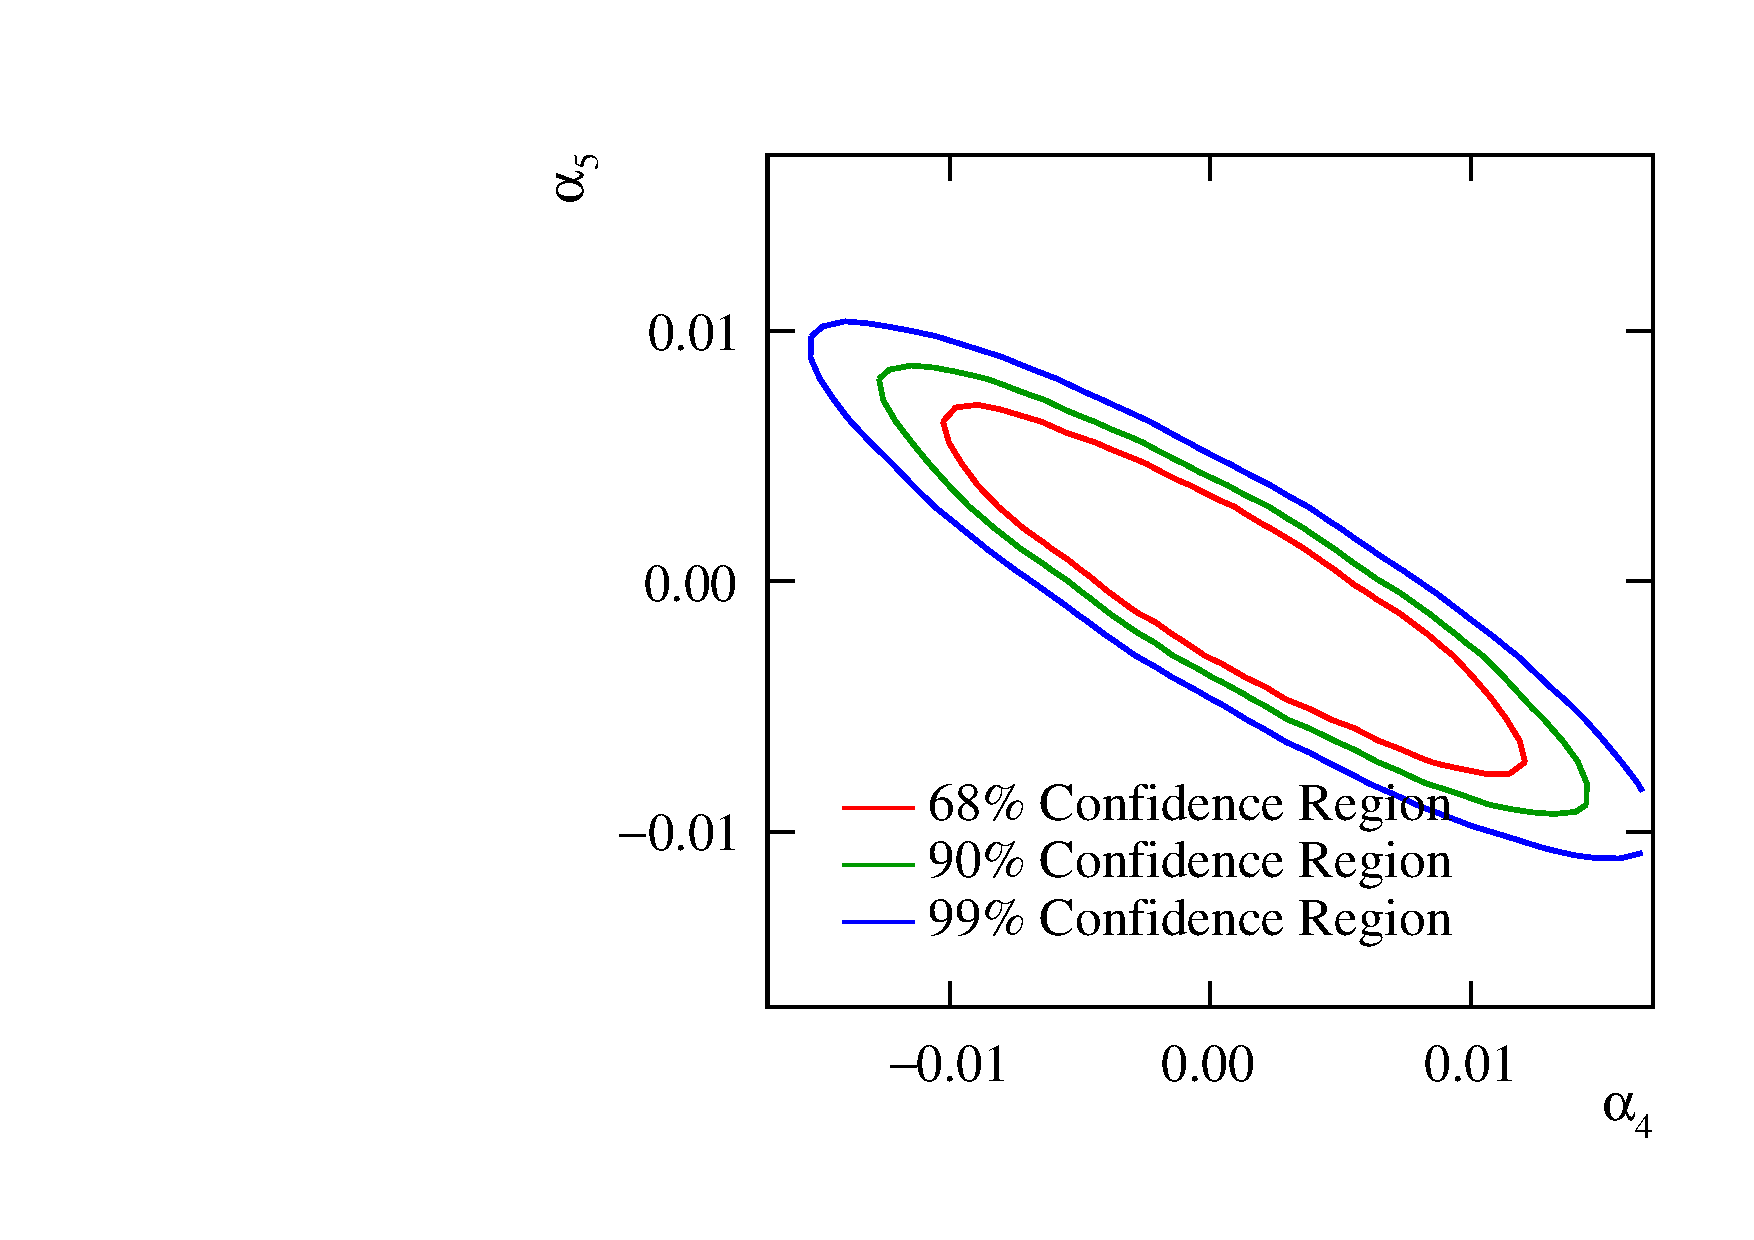
\includegraphics[width=0.3\textwidth]{PhysicsAnalysis/Plots/Chi2ContoursOptimisation/1400GeV/KtLPFOsR0p70.pdf}}
\subfloat[][Longitudinally Invariant Kt Algorithm, R = 0.9, Loose Selected PFOs, 1.4 TeV Events]{\label{fig:chi2jetalgoptkt0p90lpfos1400GeV} 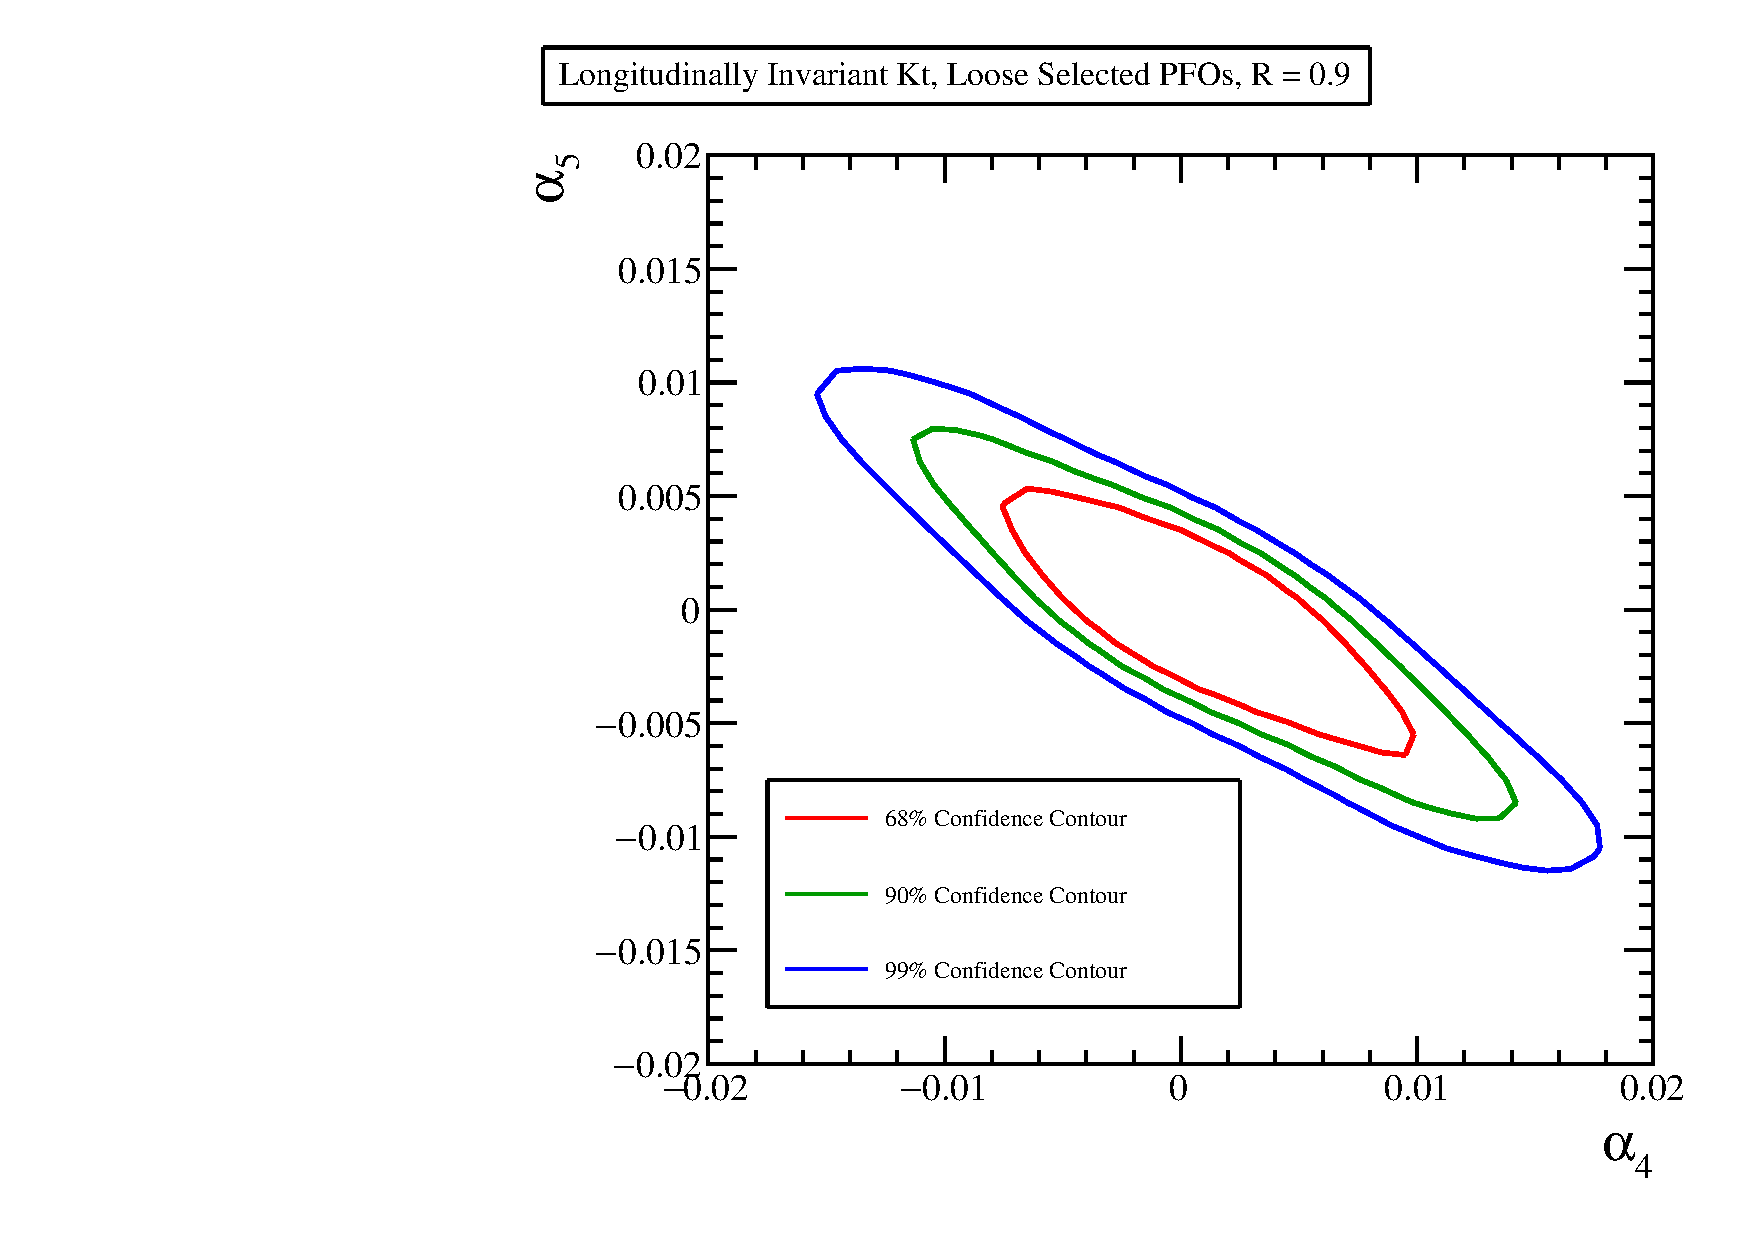
\includegraphics[width=0.3\textwidth]{PhysicsAnalysis/Plots/Chi2ContoursOptimisation/1400GeV/KtLPFOsR0p90.pdf}}
\subfloat[][Longitudinally Invariant Kt Algorithm, R = 1.1, Loose Selected PFOs, 1.4 TeV Events]{\label{fig:chi2jetalgoptkt1p10lpfos1400GeV} 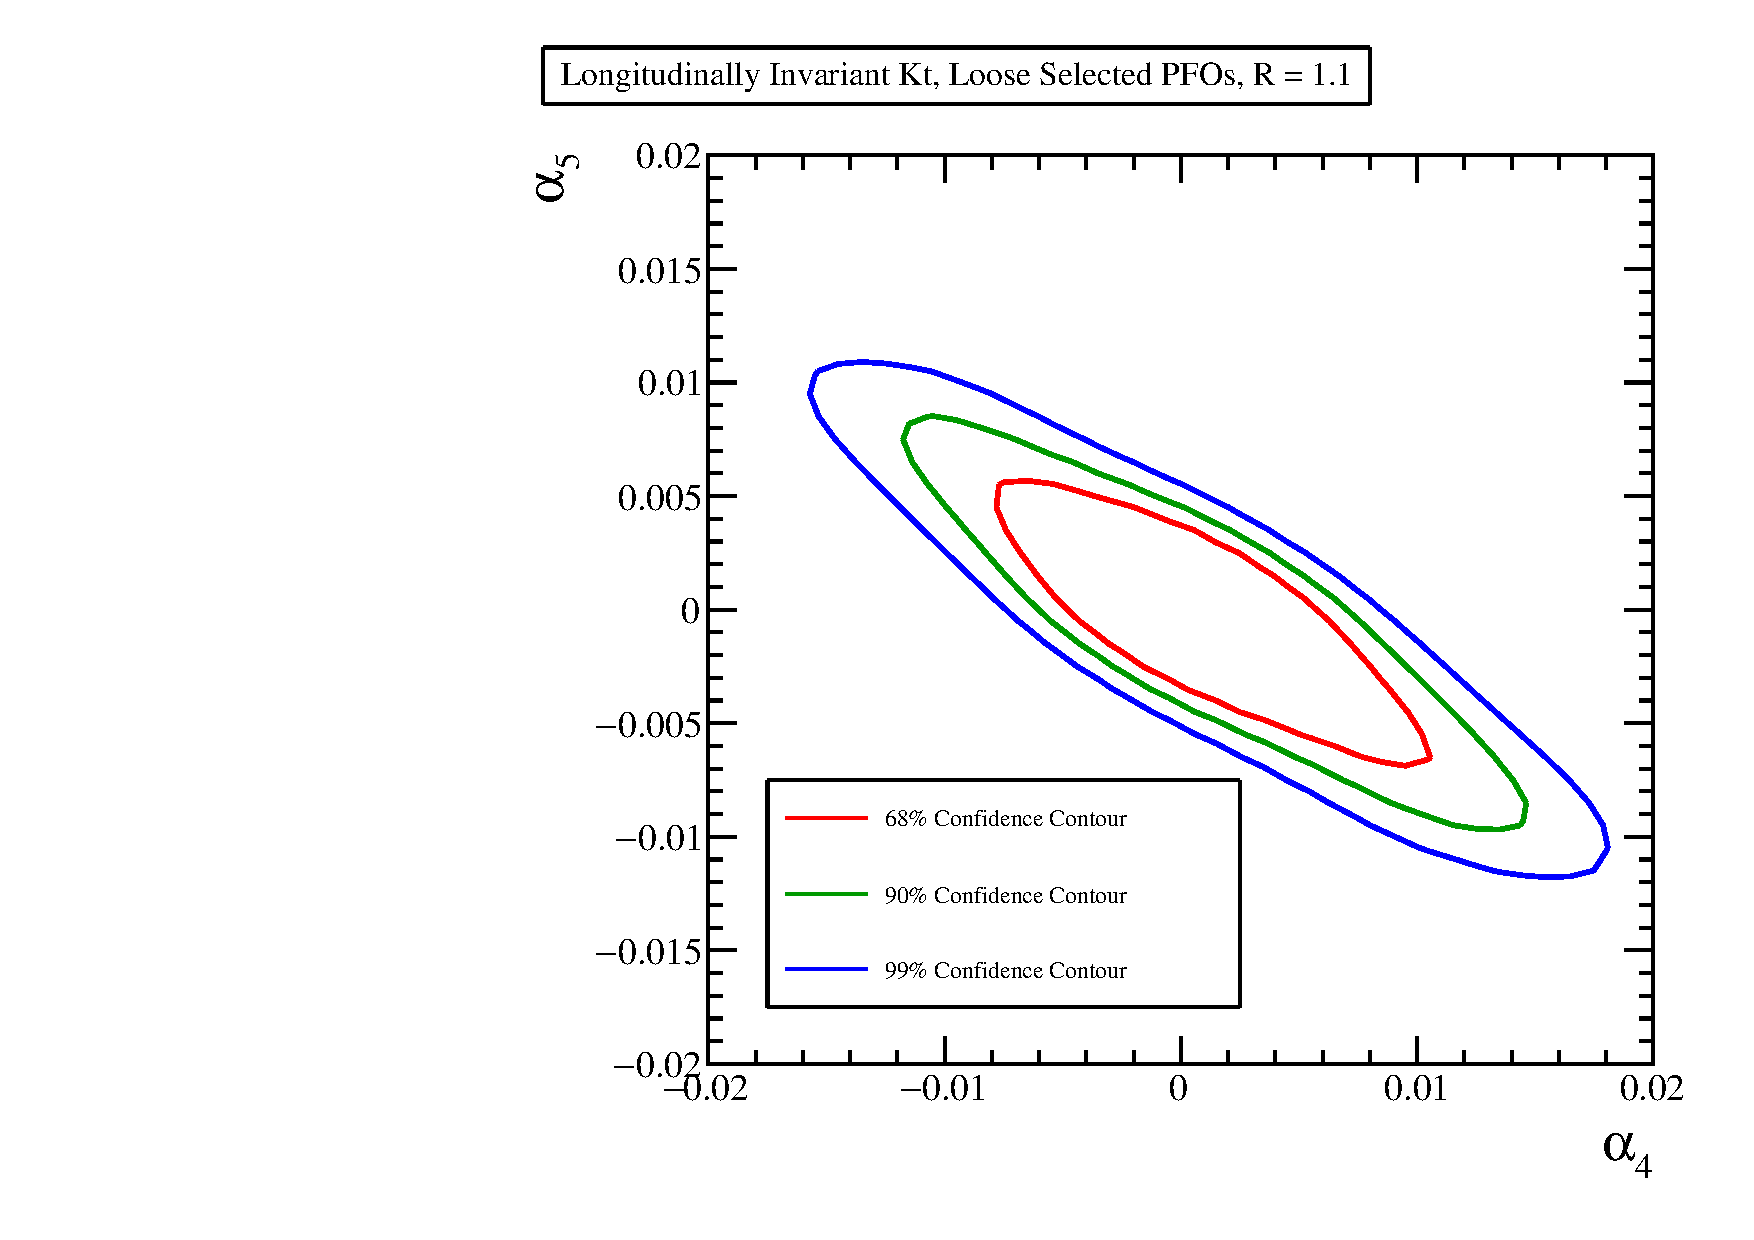
\includegraphics[width=0.3\textwidth]{PhysicsAnalysis/Plots/Chi2ContoursOptimisation/1400GeV/KtLPFOsR1p10.pdf}}\hfill
\subfloat[][Longitudinally Invariant Kt Algorithm, R = 0.7, Selected PFOs, 1.4 TeV Events]{\label{fig:chi2jetalgoptkt0p70spfos1400GeV} 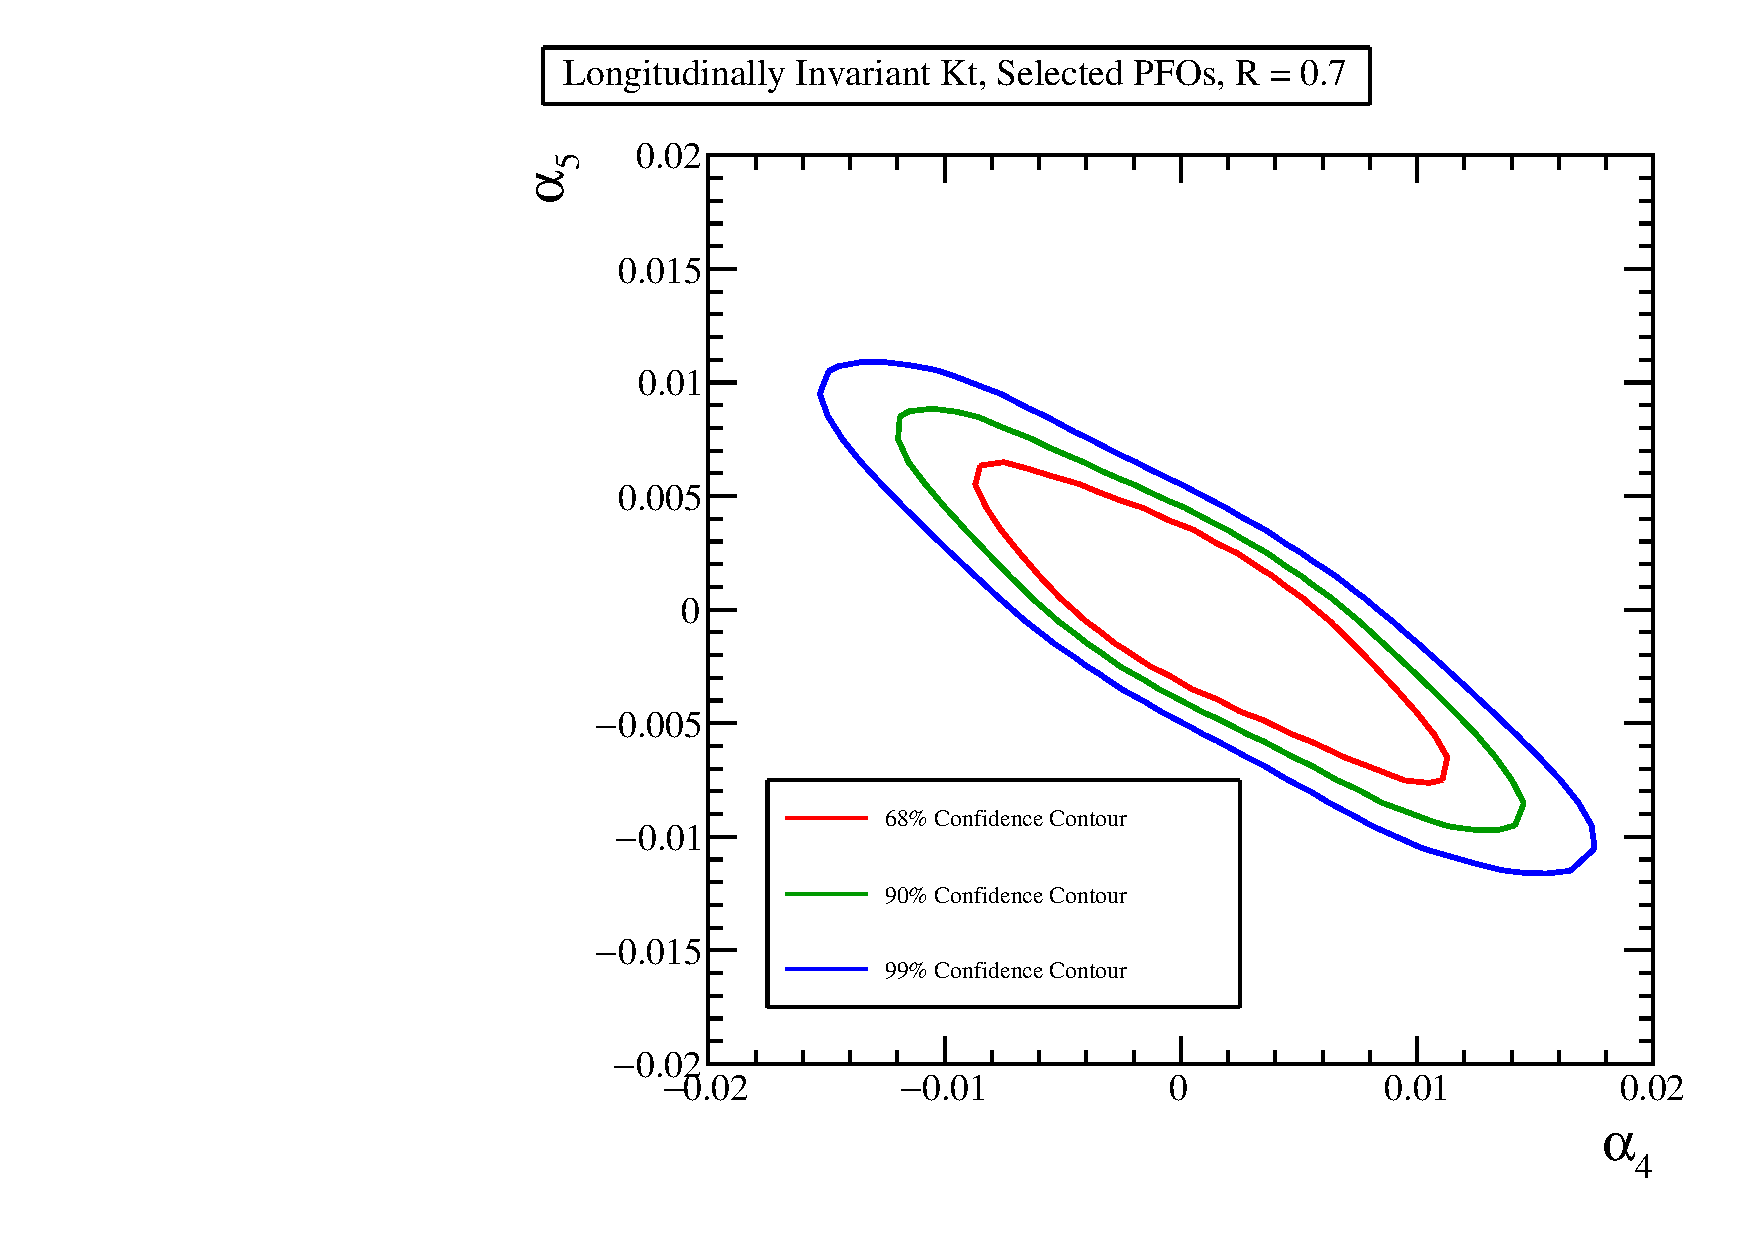
\includegraphics[width=0.3\textwidth]{PhysicsAnalysis/Plots/Chi2ContoursOptimisation/1400GeV/KtSPFOsR0p70.pdf}}
\subfloat[][Longitudinally Invariant Kt Algorithm, R = 0.9, Selected PFOs, 1.4 TeV Events]{\label{fig:chi2jetalgoptkt0p90spfos1400GeV} 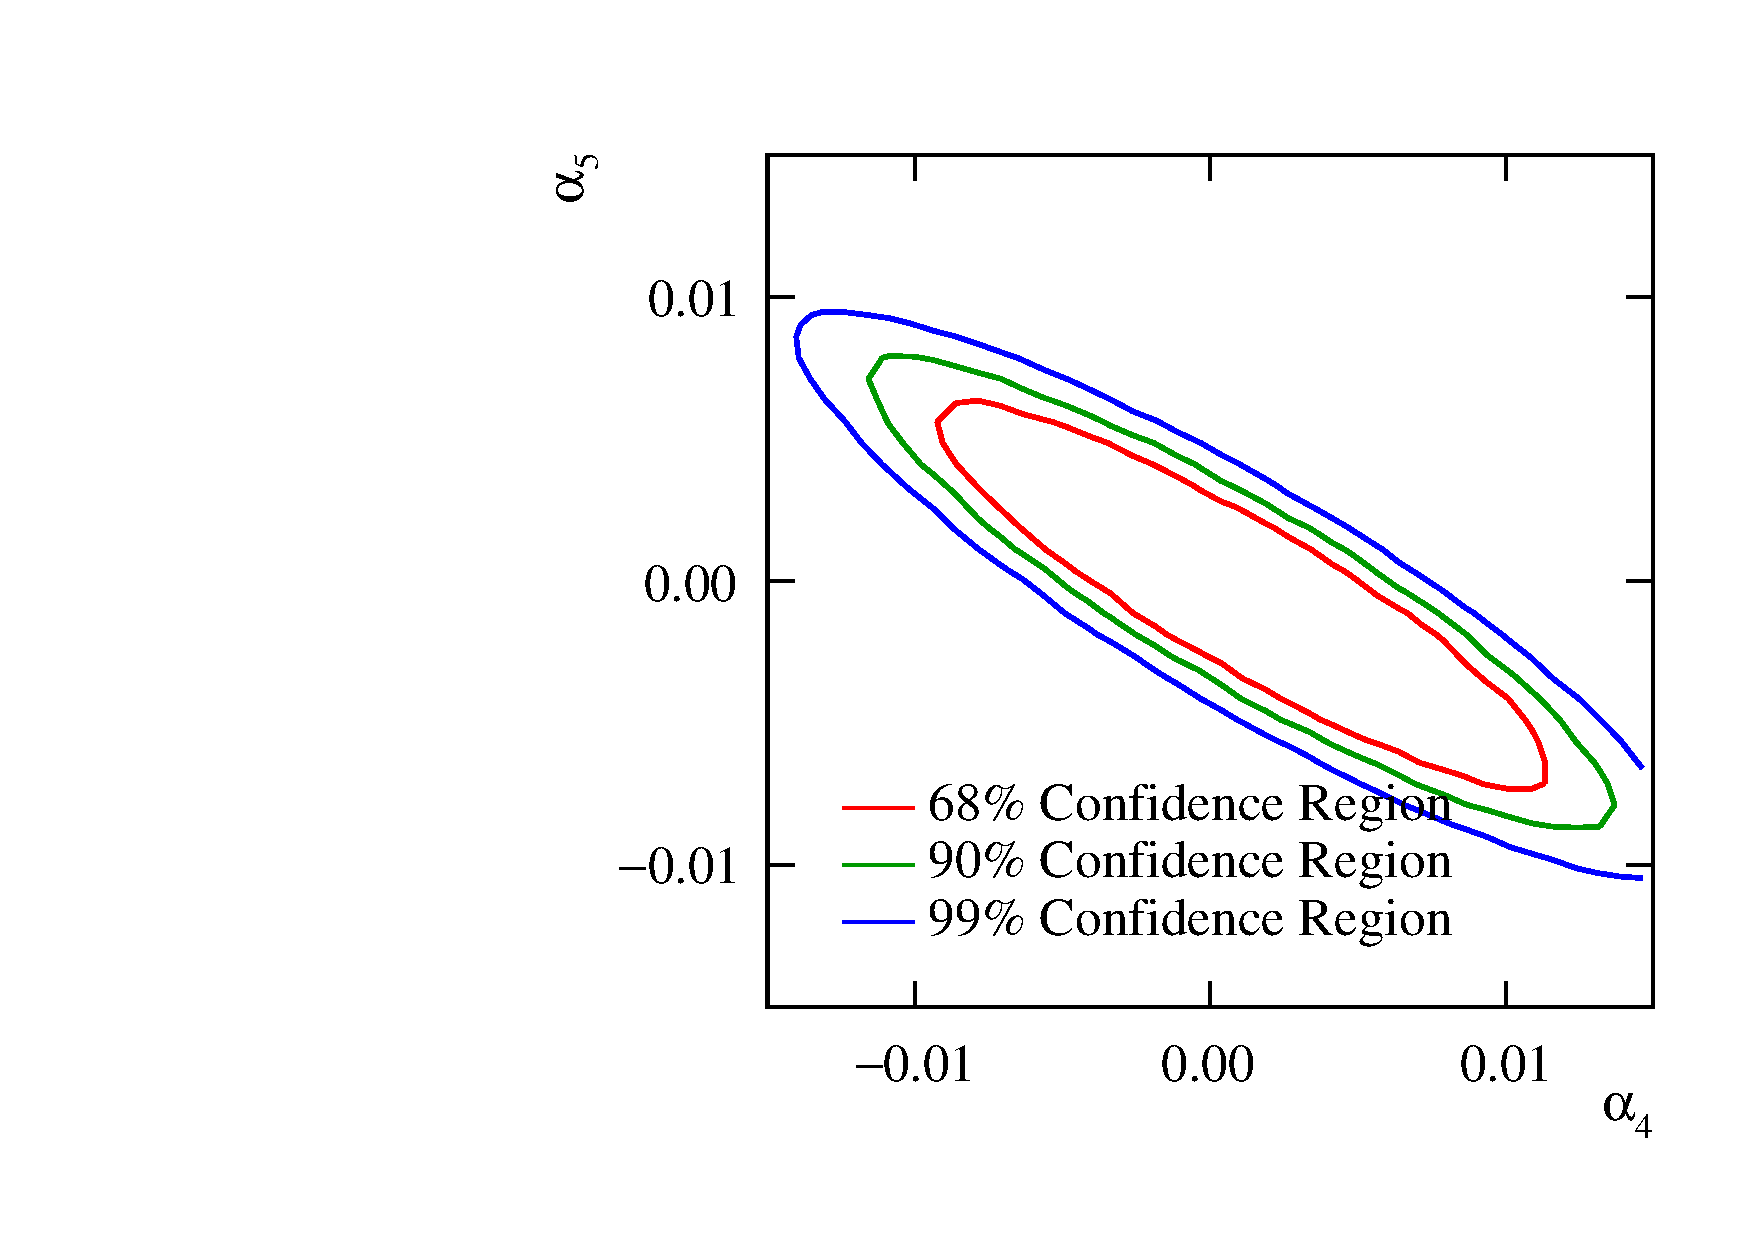
\includegraphics[width=0.3\textwidth]{PhysicsAnalysis/Plots/Chi2ContoursOptimisation/1400GeV/KtSPFOsR0p90.pdf}}
\subfloat[][Longitudinally Invariant Kt Algorithm, R = 1.1, Selected PFOs, 1.4 TeV Events]{\label{fig:chi2jetalgoptkt1p10spfos1400GeV} 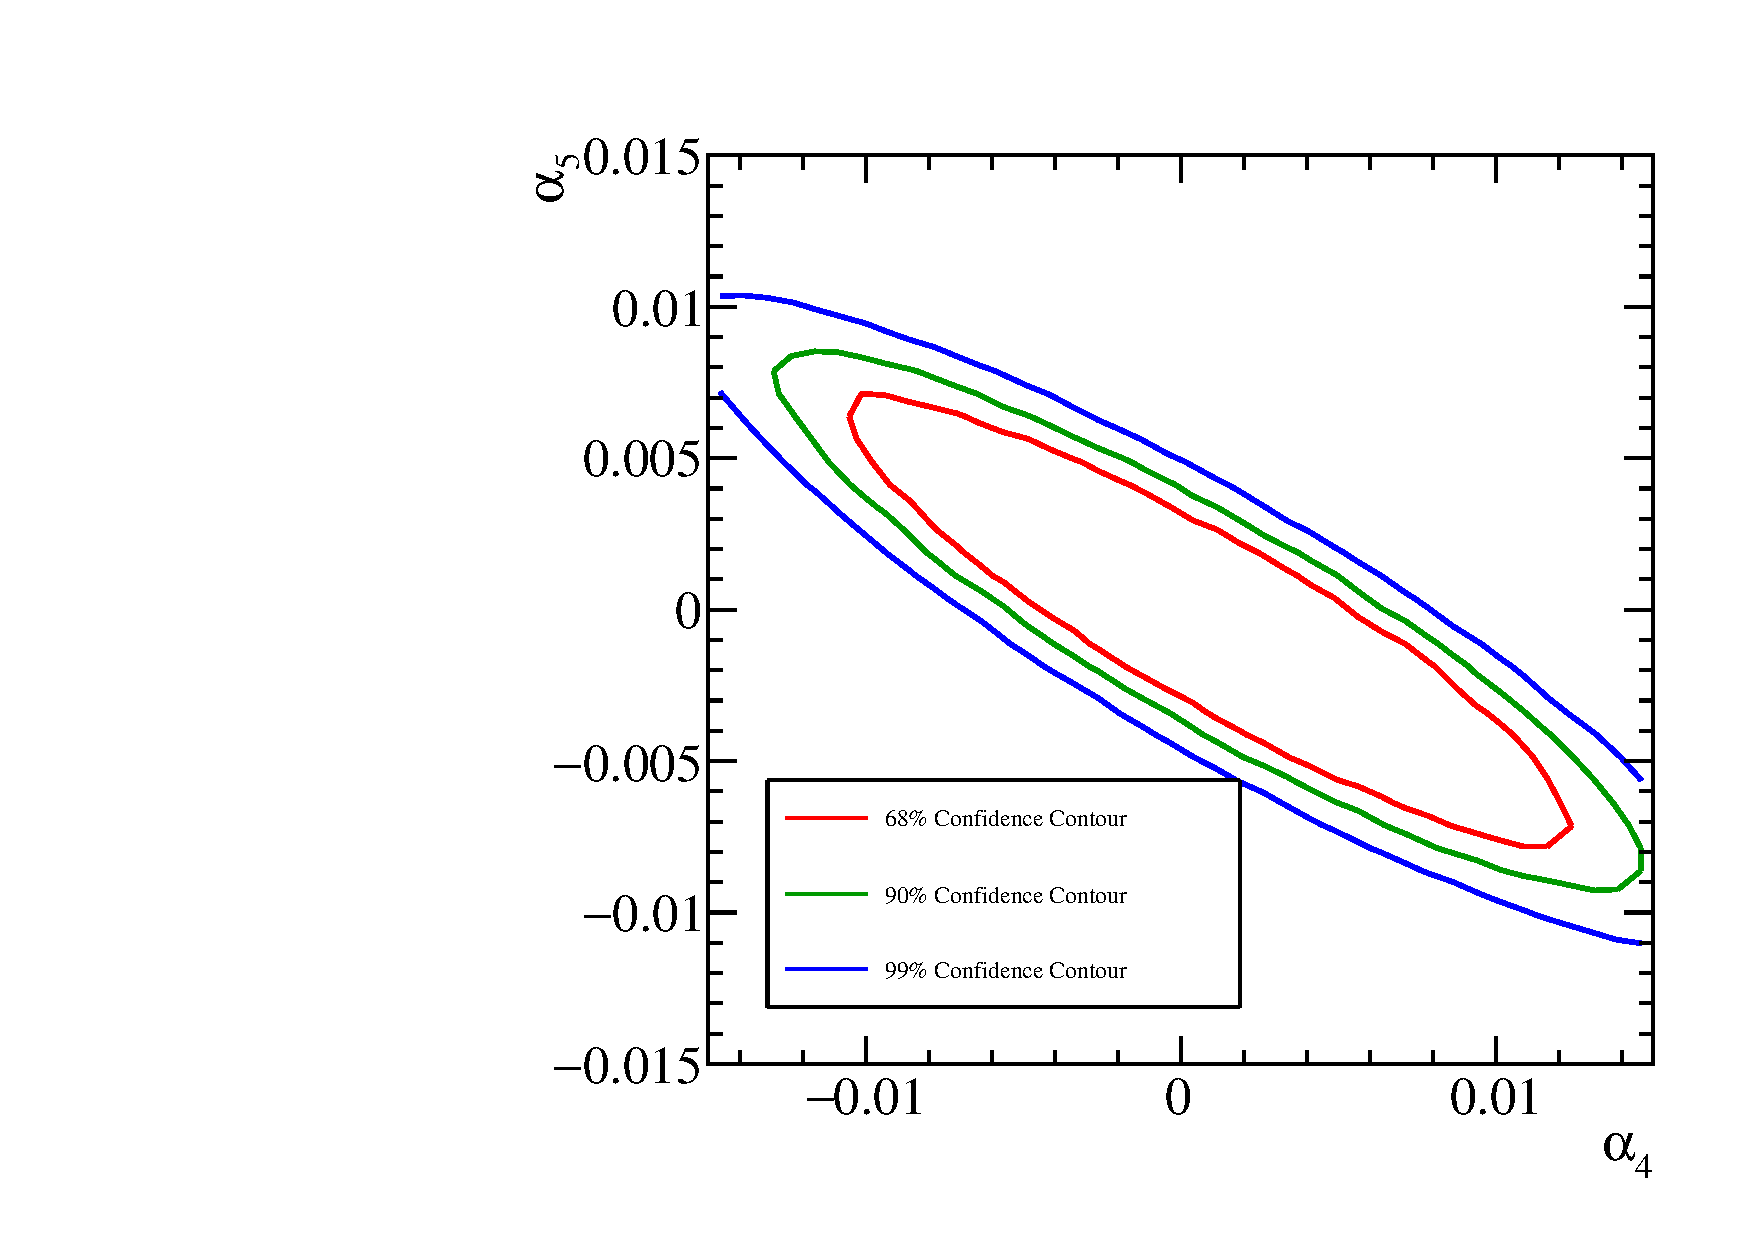
\includegraphics[width=0.3\textwidth]{PhysicsAnalysis/Plots/Chi2ContoursOptimisation/1400GeV/KtSPFOsR1p10.pdf}}\hfill
\subfloat[][Longitudinally Invariant Kt Algorithm, R = 0.7, Tight Selected PFOs, 1.4 TeV Events]{\label{fig:chi2jetalgoptkt0p70tpfos1400GeV} 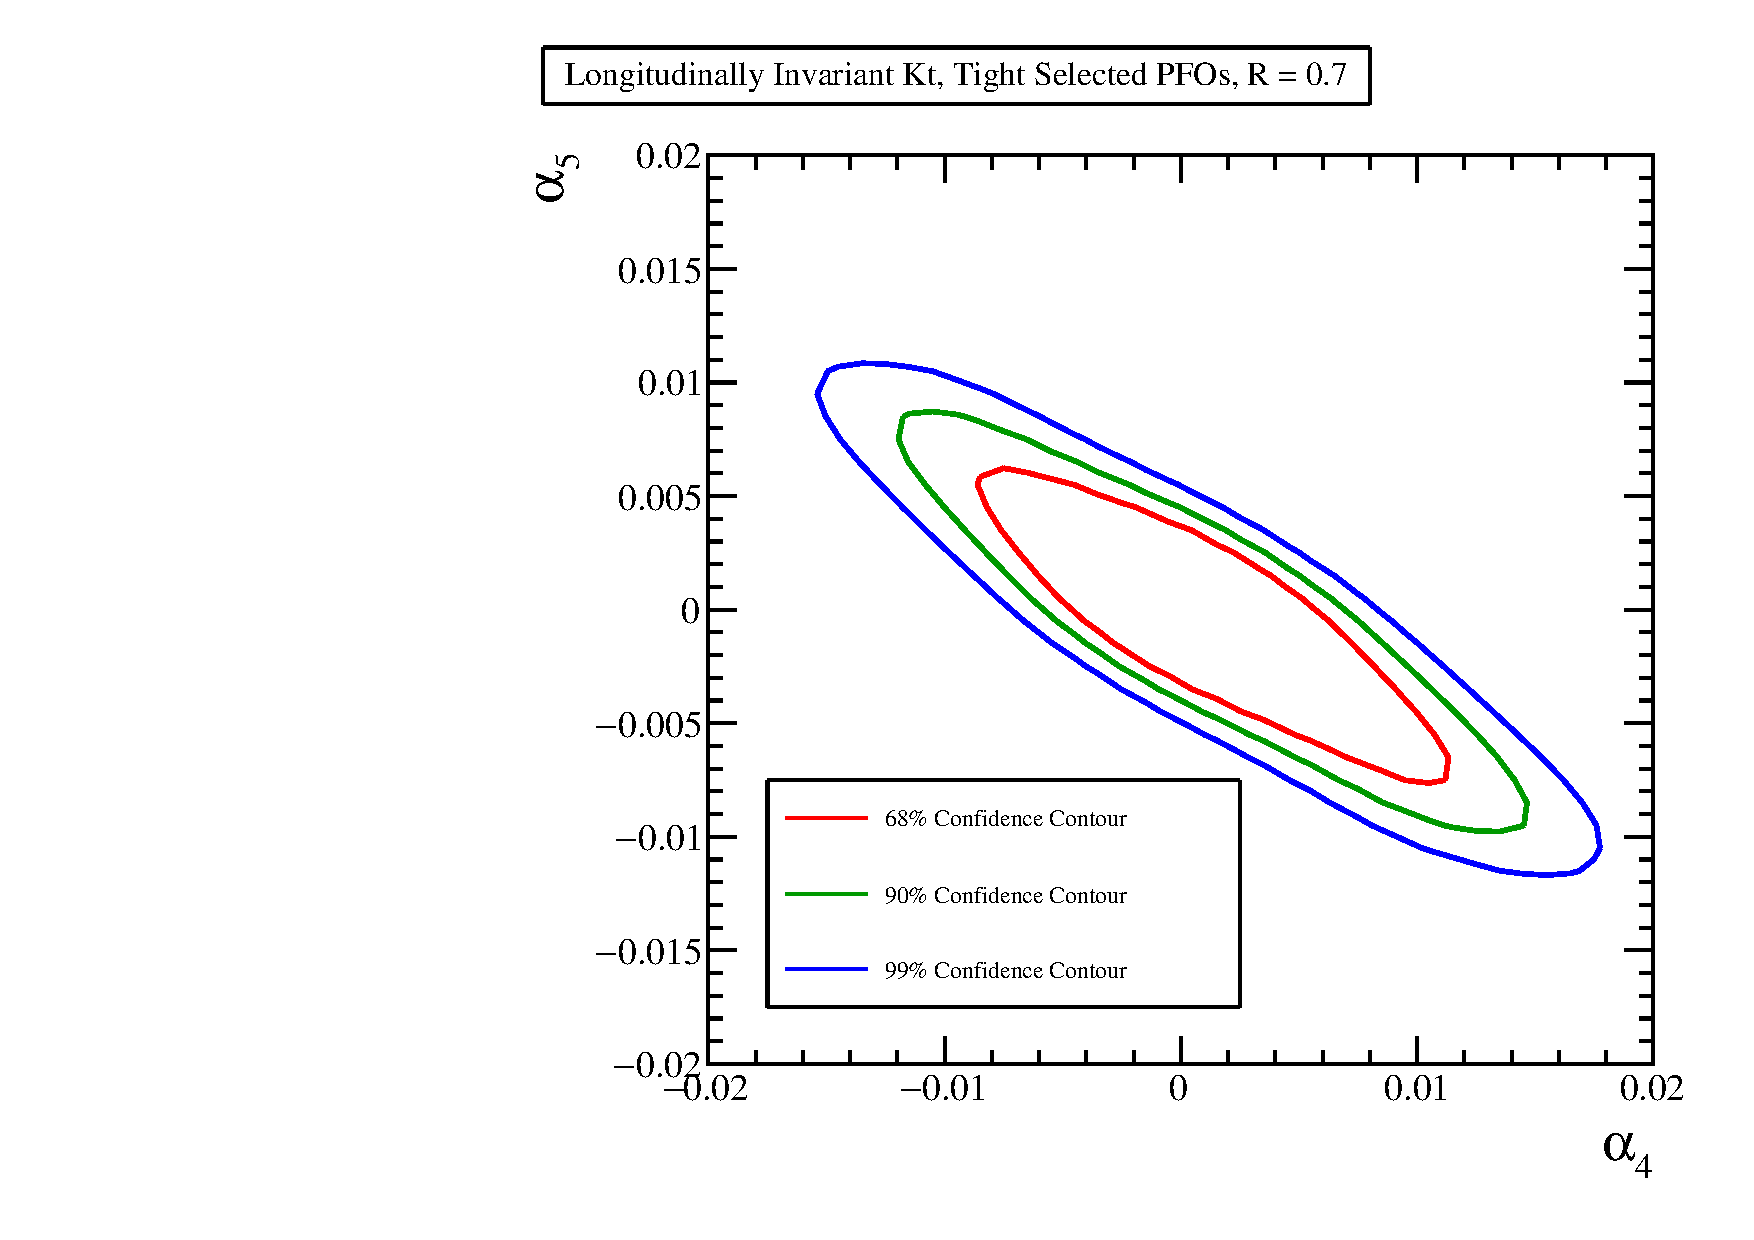
\includegraphics[width=0.3\textwidth]{PhysicsAnalysis/Plots/Chi2ContoursOptimisation/1400GeV/KtTPFOsR0p70.pdf}}
\subfloat[][Longitudinally Invariant Kt Algorithm, R = 0.9, Tight Selected PFOs, 1.4 TeV Events]{\label{fig:chi2jetalgoptkt0p90tpfos1400GeV} 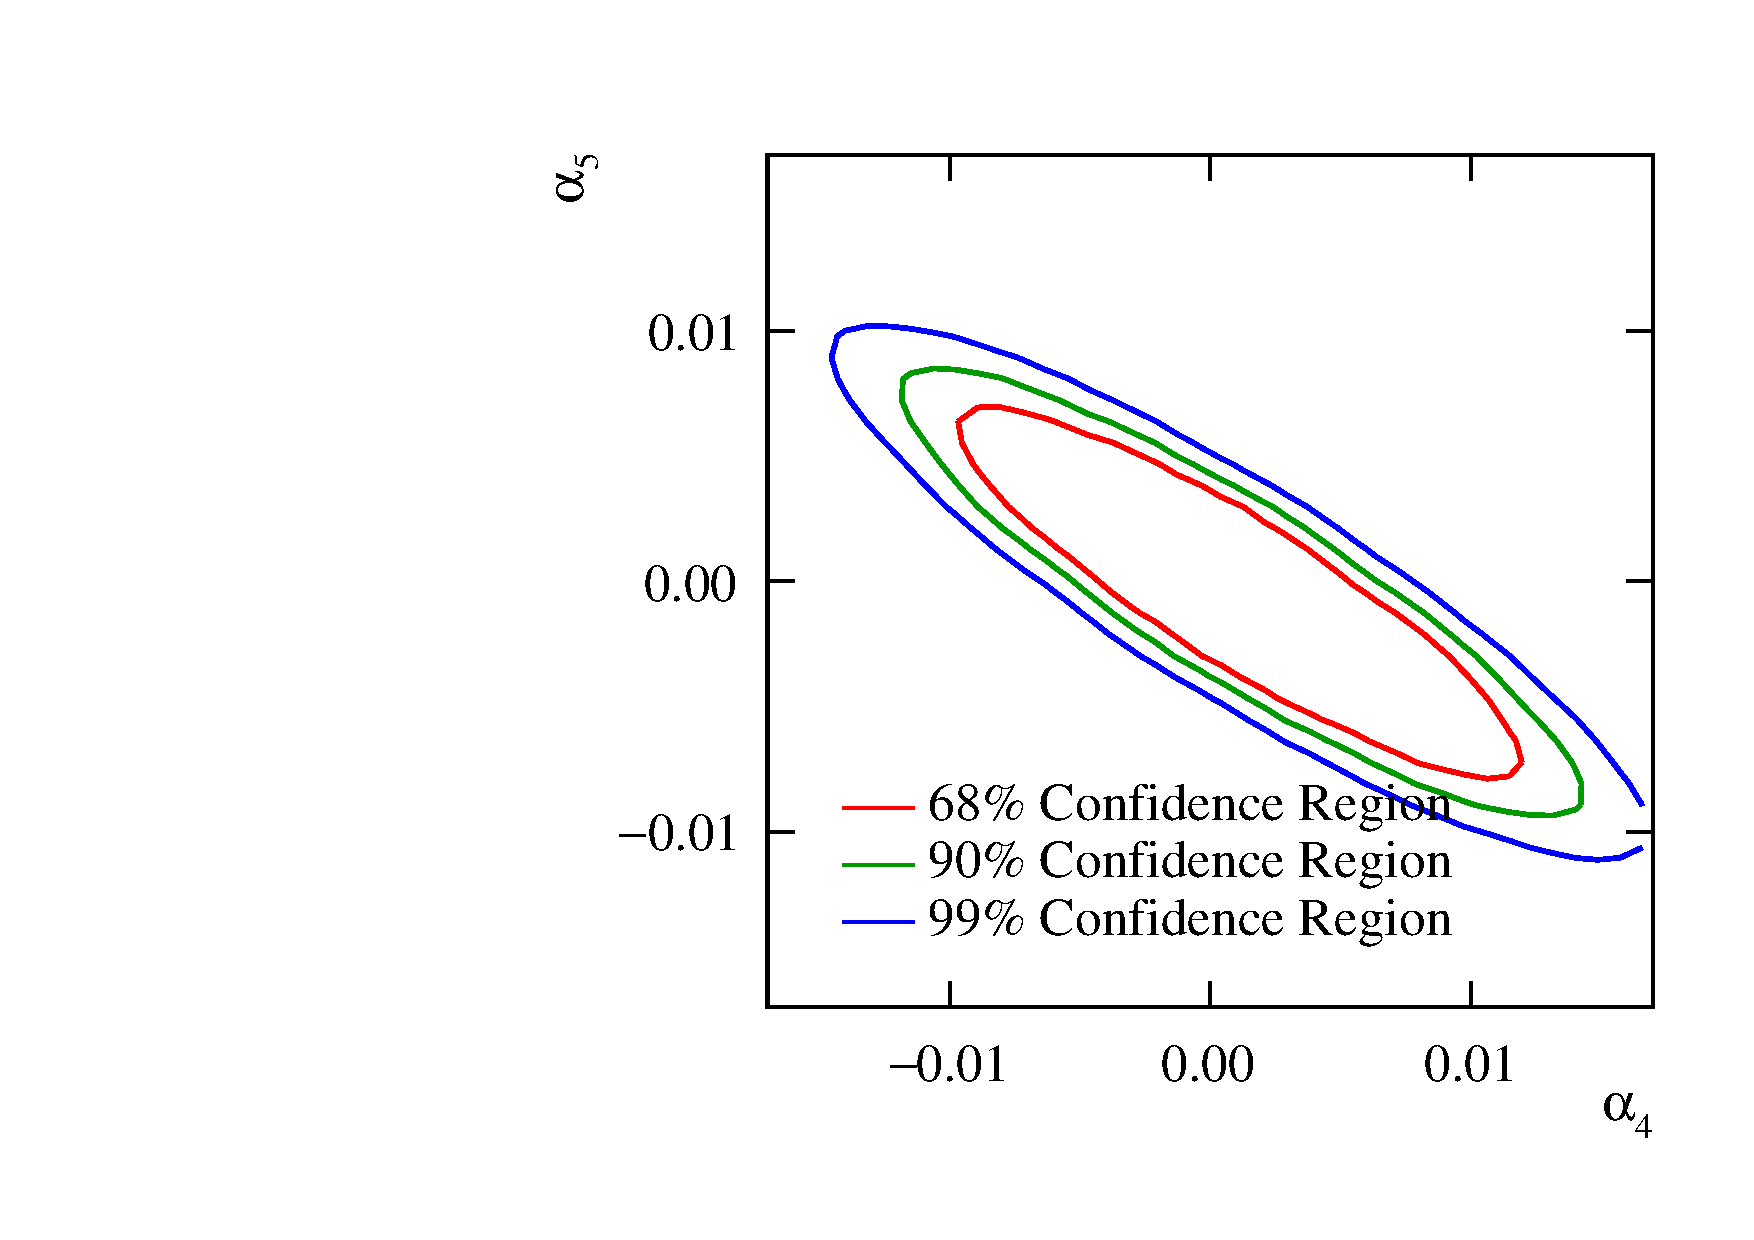
\includegraphics[width=0.3\textwidth]{PhysicsAnalysis/Plots/Chi2ContoursOptimisation/1400GeV/KtTPFOsR0p90.pdf}}
\subfloat[][Longitudinally Invariant Kt Algorithm, R = 1.1, Tight Selected PFOs, 1.4 TeV Events]{\label{fig:chi2jetalgoptkt1p10tpfos1400GeV} 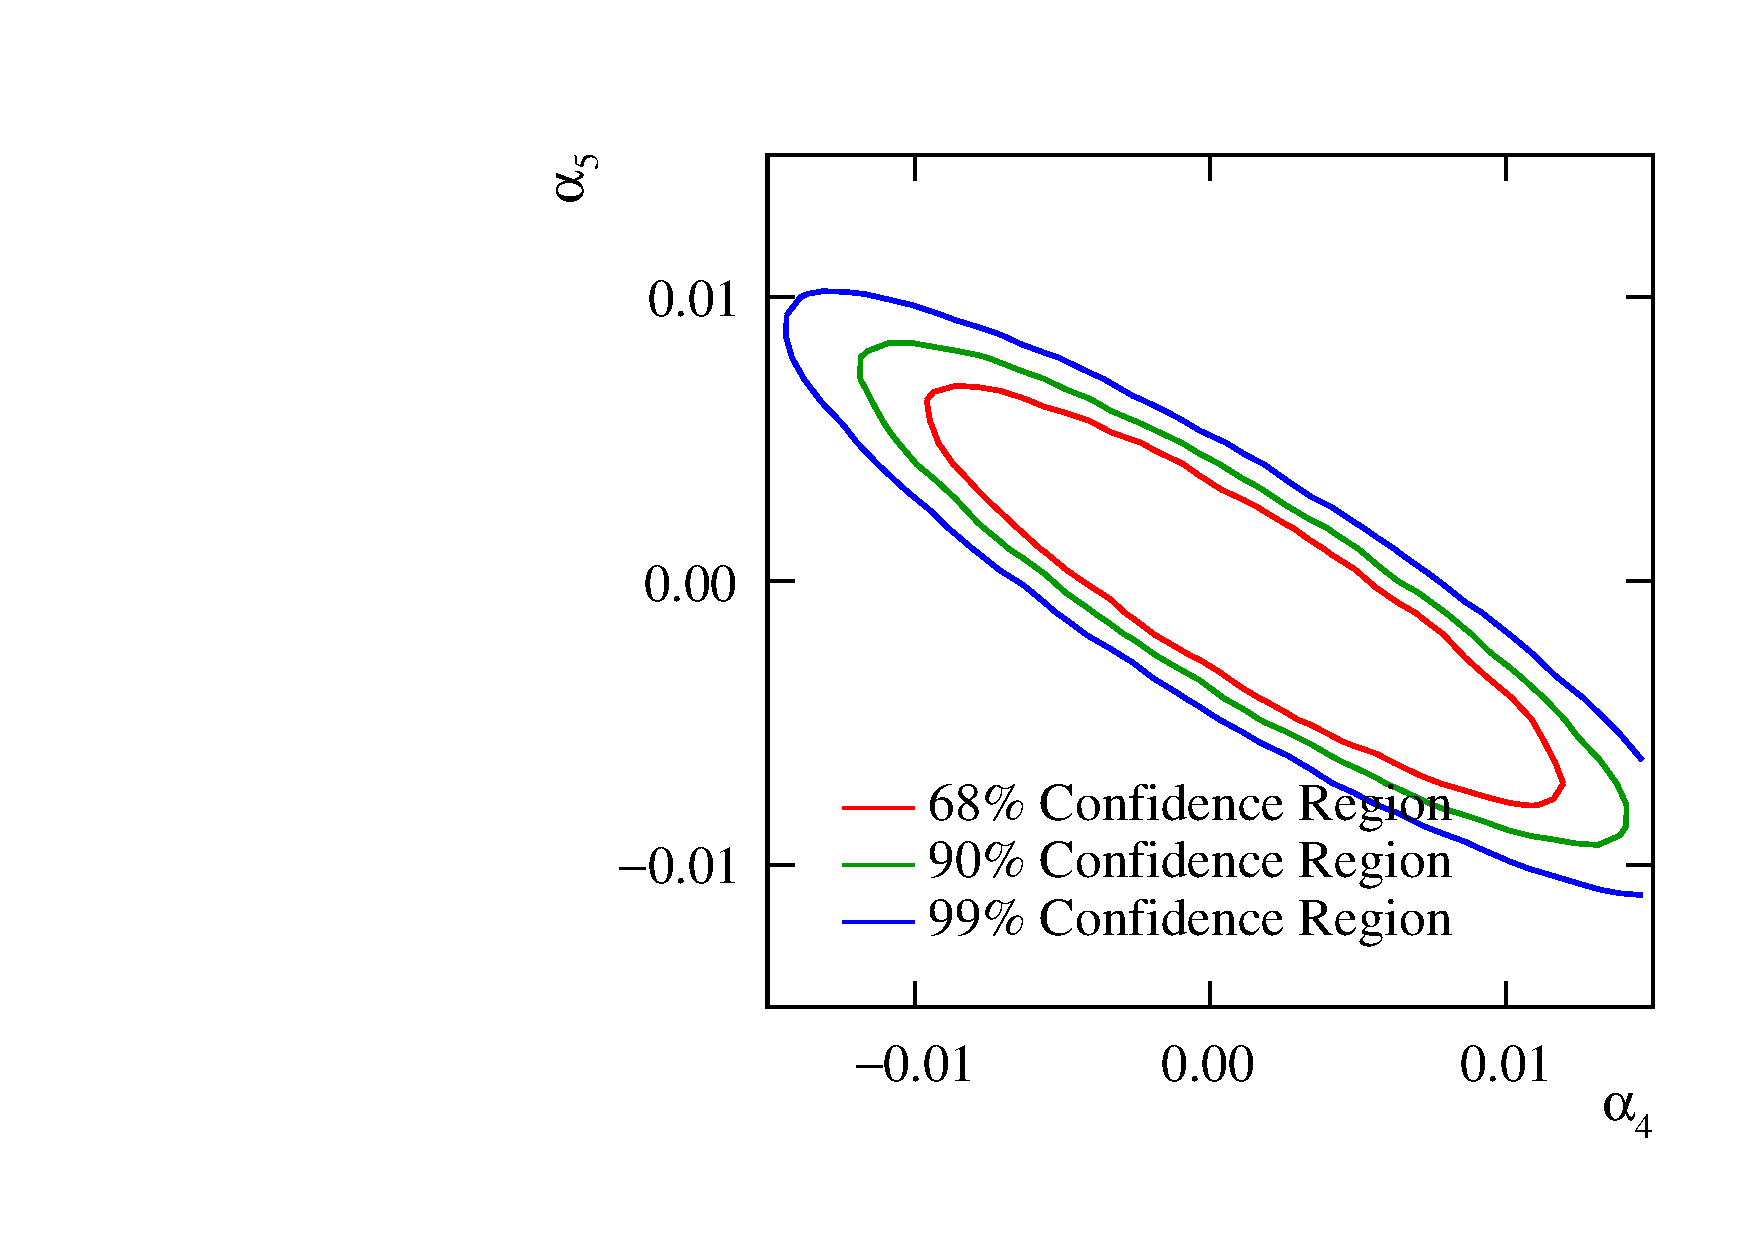
\includegraphics[width=0.3\textwidth]{PhysicsAnalysis/Plots/Chi2ContoursOptimisation/1400GeV/KtTPFOsR1p10.pdf}}\hfill
\caption[$\chi^{2}$ Sensitivity contours for the $\text{qqqq}\nu\nu$ final state arising from a fit to $\text{cos}\theta^{*}_{\text{Jets}}$ at 1.4 TeV for different values of jet reconstruction parameters.]{$\chi^{2}$ Sensitivity contours for the $\text{qqqq}\nu\nu$ final state arising from a fit to $\text{cos}\theta^{*}_{\text{Jets}}$ at 1.4 TeV for different values of jet reconstruction parameters.}
\label{fig:chi2jetalgopt1400GeV}
\end{figure}

\begin{figure}
\subfloat[][Longitudinally Invariant Kt Algorithm, R = 0.7, Loose Selected PFOs, 3 TeV Events]{\label{fig:chi2jetalgoptkt0p70lpfos3000GeV} 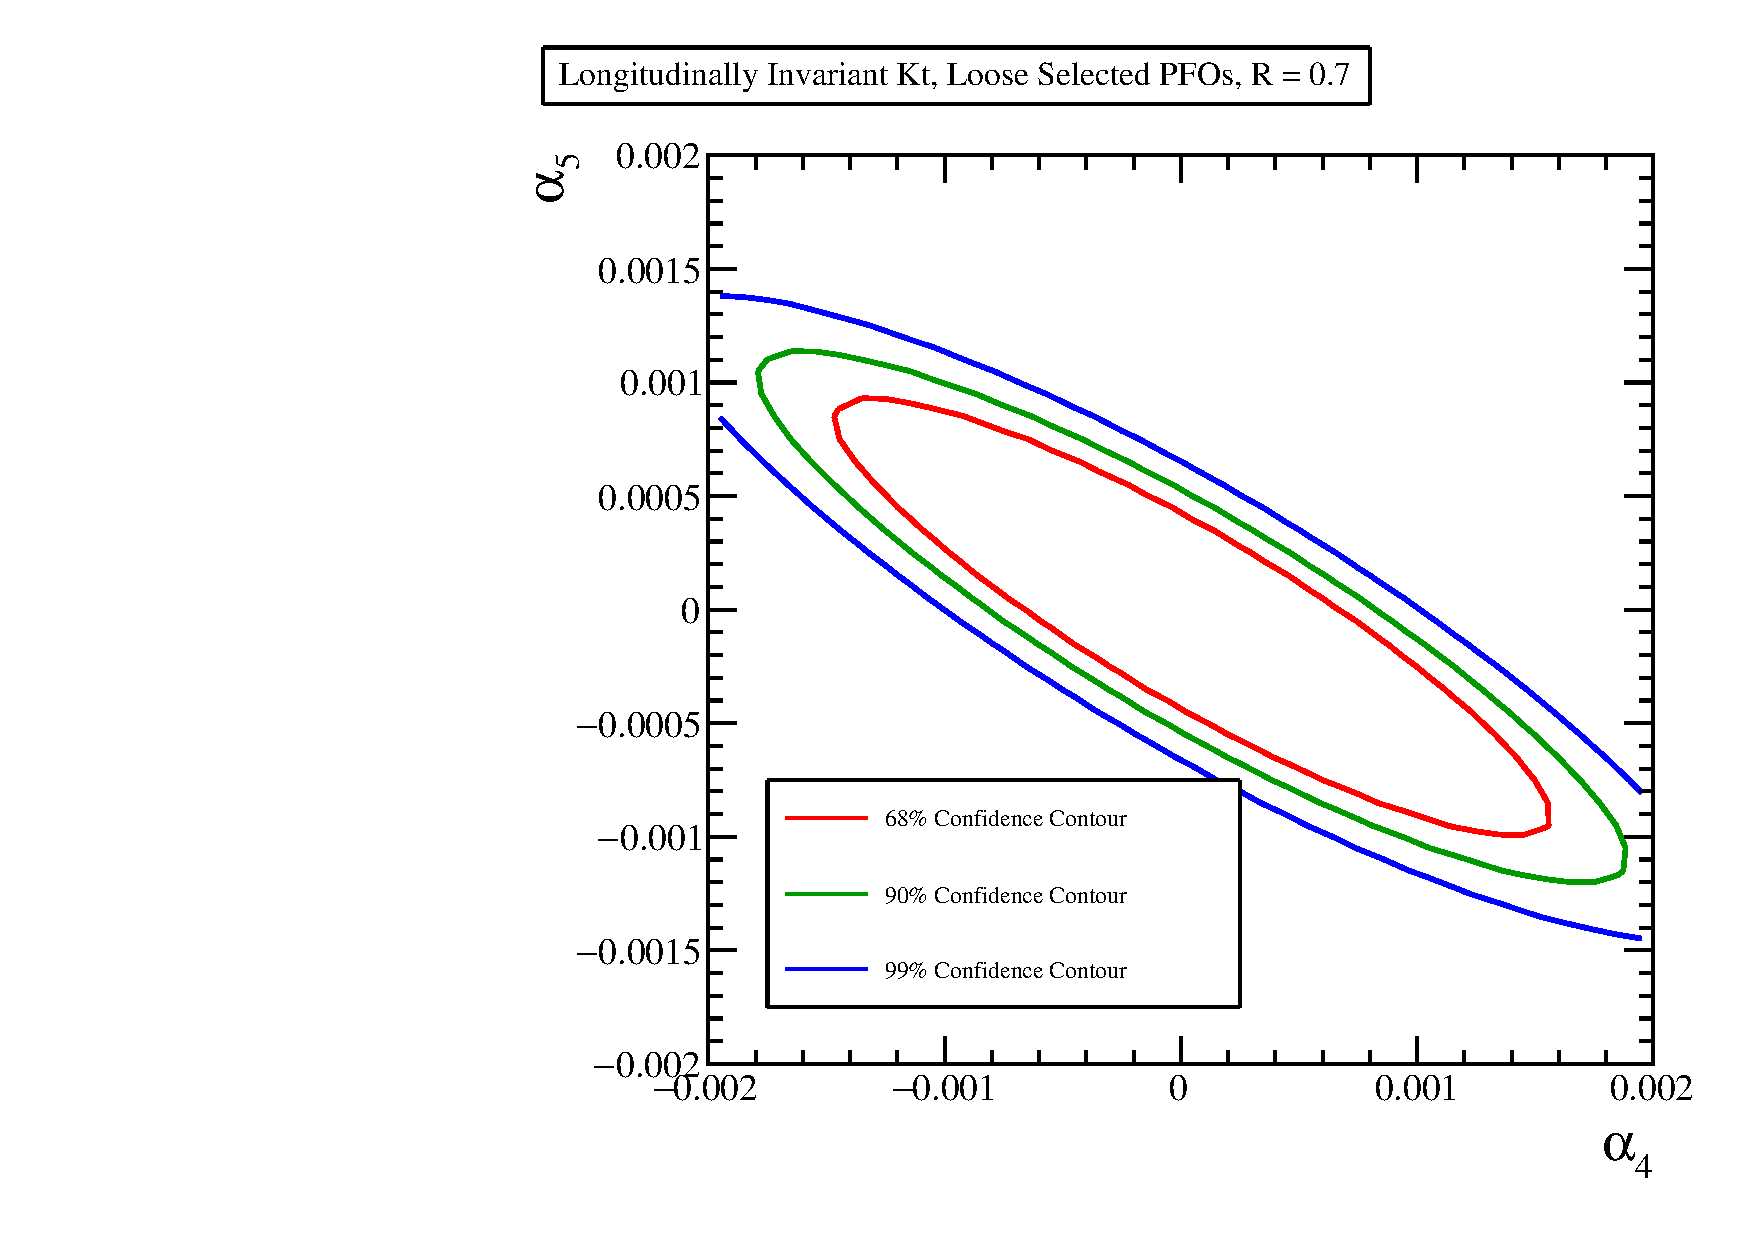
\includegraphics[width=0.3\textwidth]{PhysicsAnalysis/Plots/Chi2ContoursOptimisation/3000GeV/KtLPFOsR0p70.pdf}}
\subfloat[][Longitudinally Invariant Kt Algorithm, R = 0.9, Loose Selected PFOs, 3 TeV Events]{\label{fig:chi2jetalgoptkt0p90lpfos3000GeV} 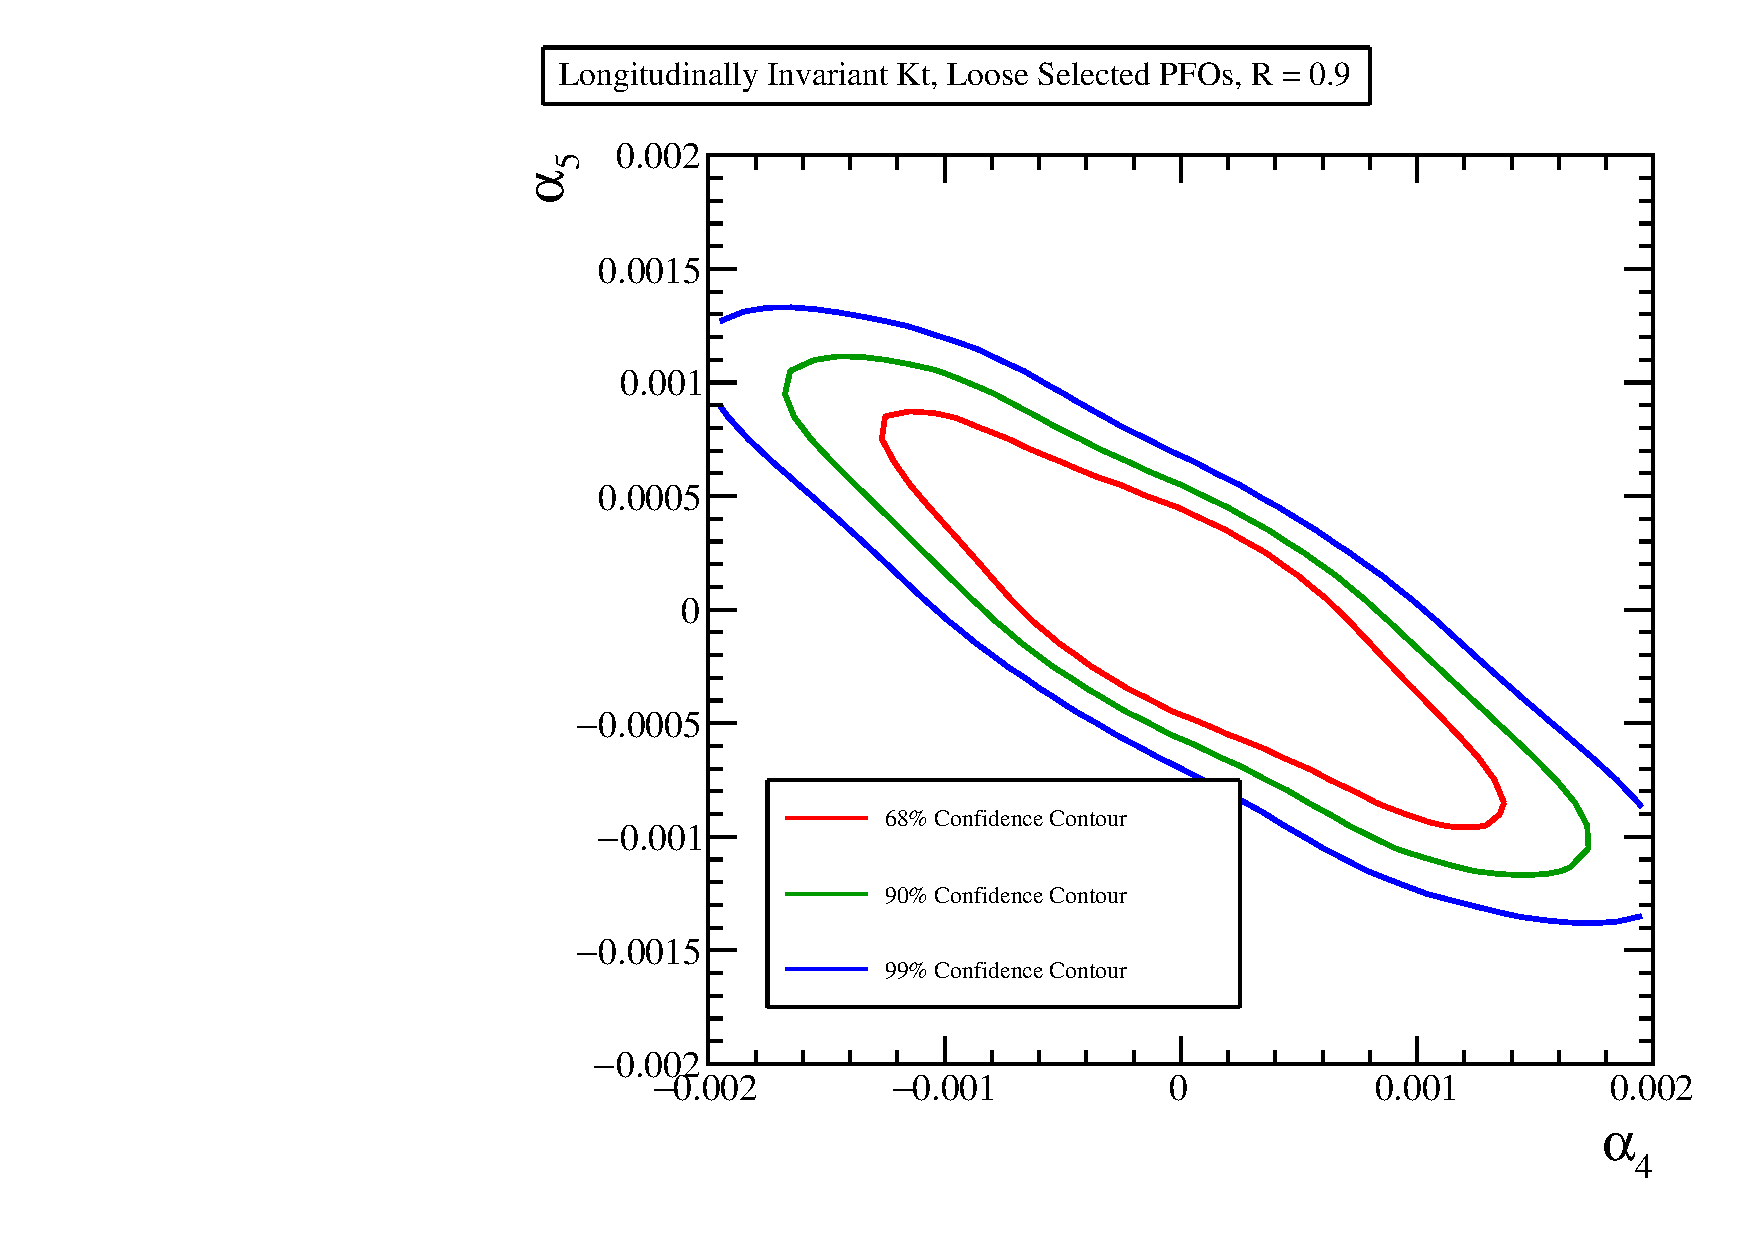
\includegraphics[width=0.3\textwidth]{PhysicsAnalysis/Plots/Chi2ContoursOptimisation/3000GeV/KtLPFOsR0p90.pdf}}
\subfloat[][Longitudinally Invariant Kt Algorithm, R = 1.1, Loose Selected PFOs, 3 TeV Events]{\label{fig:chi2jetalgoptkt1p10lpfos3000GeV} 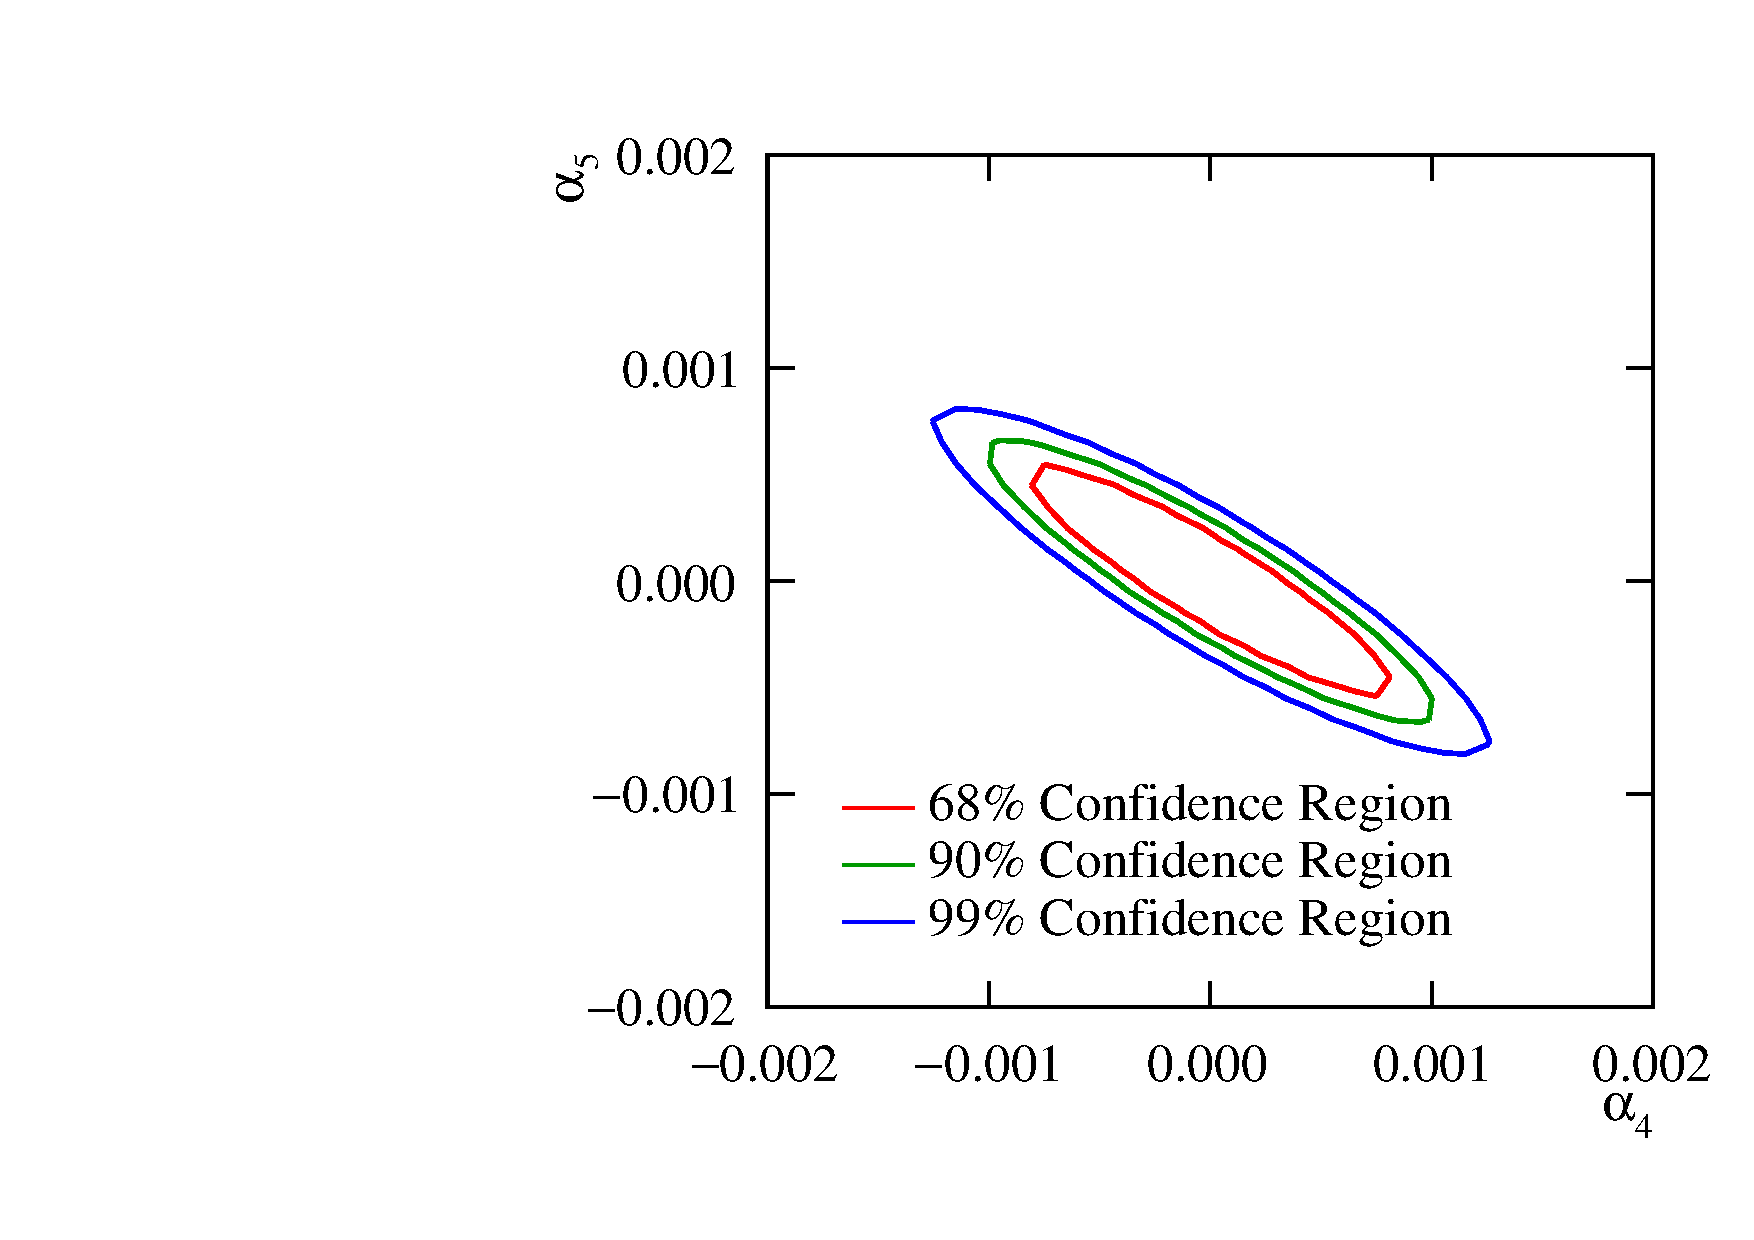
\includegraphics[width=0.3\textwidth]{PhysicsAnalysis/Plots/Chi2ContoursOptimisation/3000GeV/KtLPFOsR1p10.pdf}}\hfill
\subfloat[][Longitudinally Invariant Kt Algorithm, R = 0.7, Selected PFOs, 3 TeV Events]{\label{fig:chi2jetalgoptkt0p70spfos3000GeV} 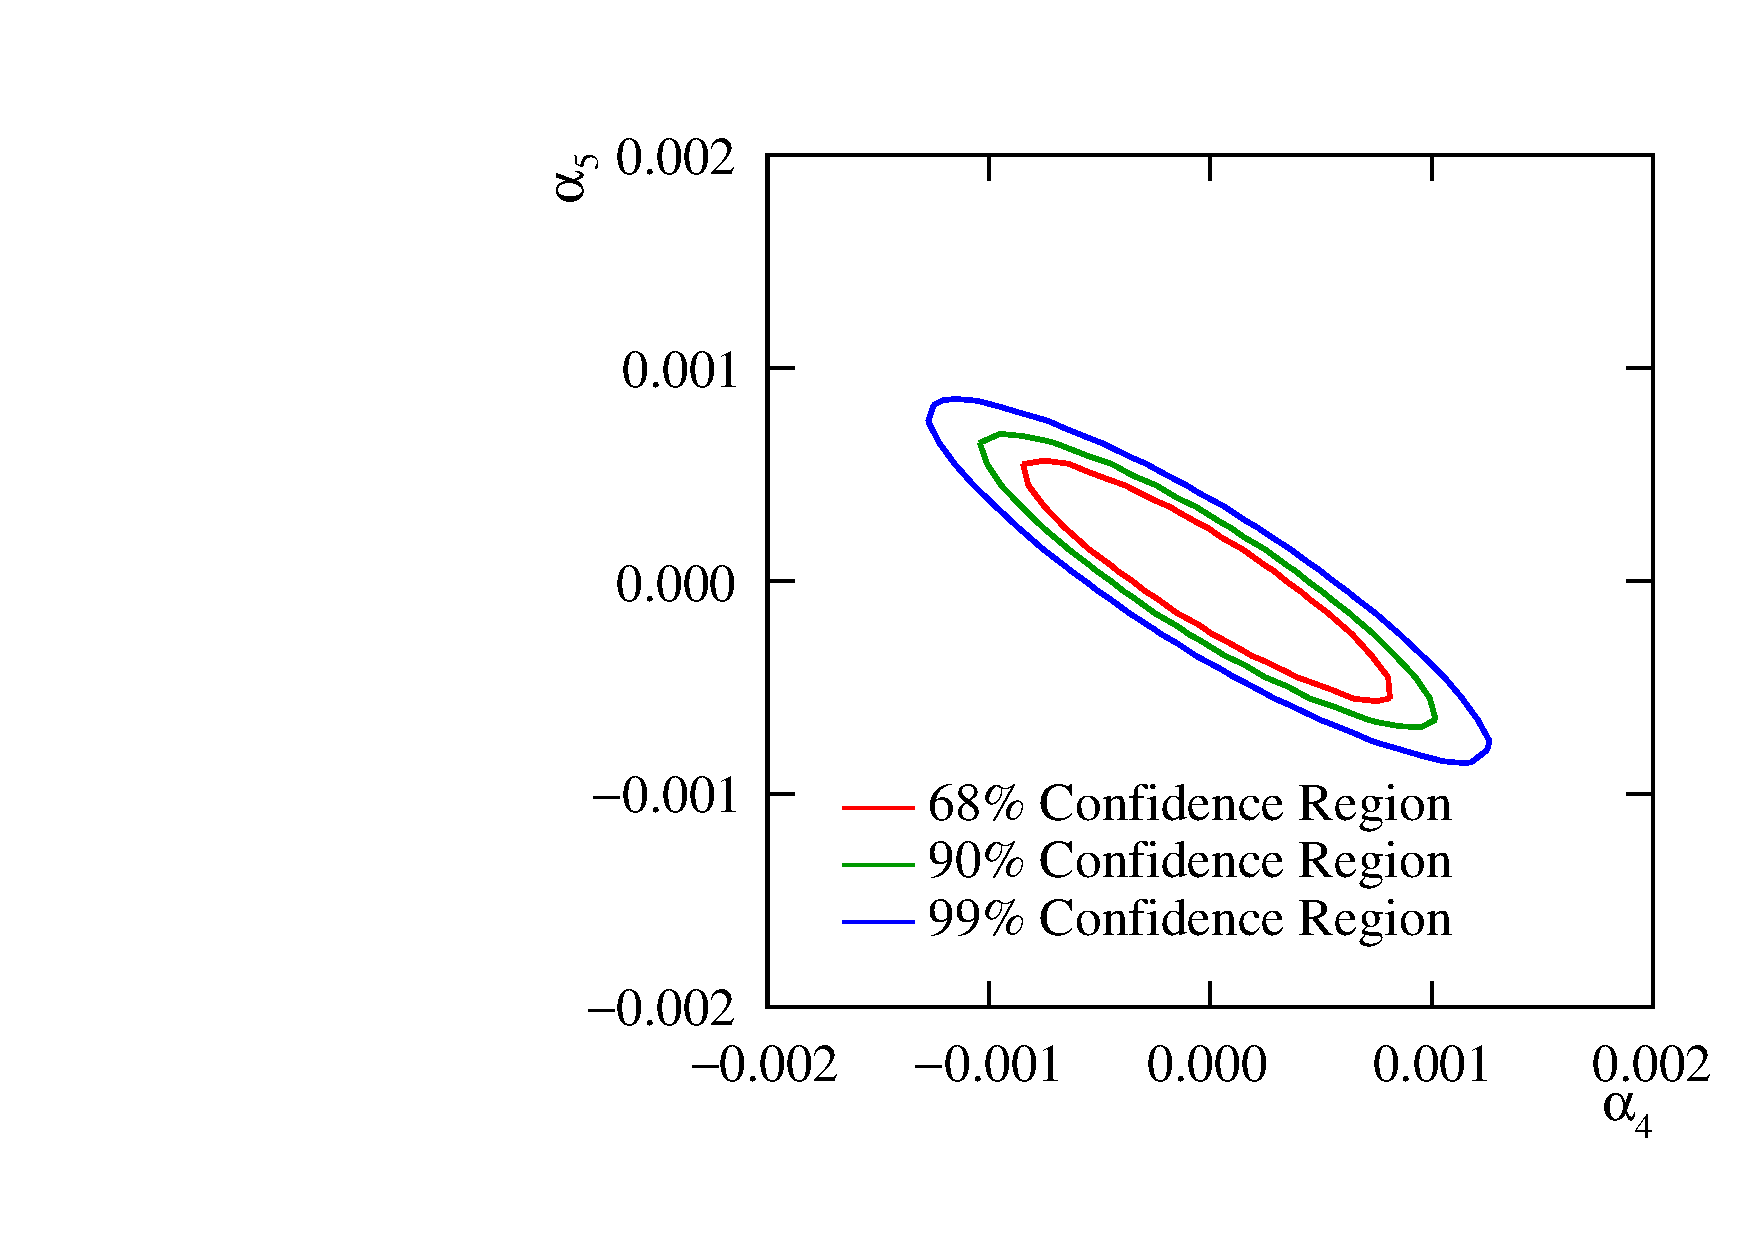
\includegraphics[width=0.3\textwidth]{PhysicsAnalysis/Plots/Chi2ContoursOptimisation/3000GeV/KtSPFOsR0p70.pdf}}
\subfloat[][Longitudinally Invariant Kt Algorithm, R = 0.9, Selected PFOs, 3 TeV Events]{\label{fig:chi2jetalgoptkt0p90spfos3000GeV} 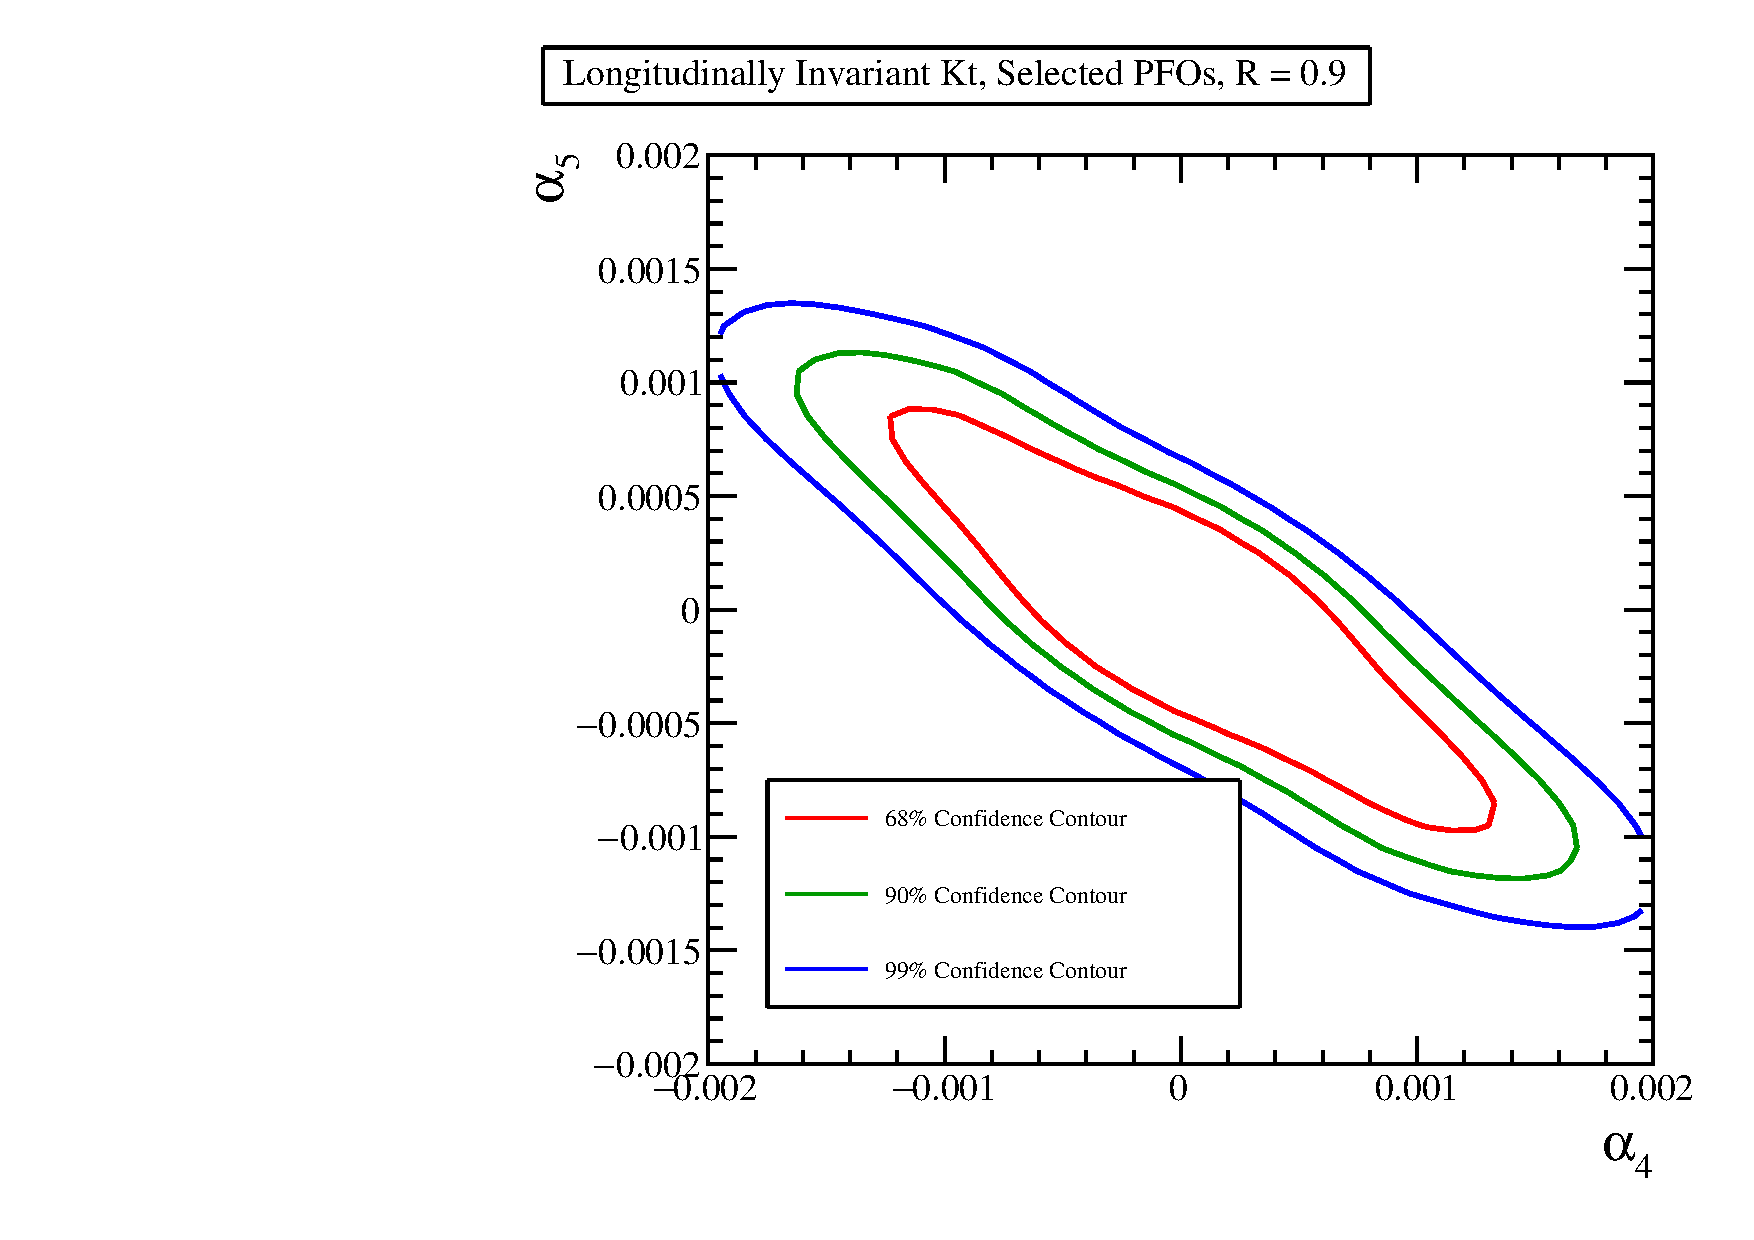
\includegraphics[width=0.3\textwidth]{PhysicsAnalysis/Plots/Chi2ContoursOptimisation/3000GeV/KtSPFOsR0p90.pdf}}
\subfloat[][Longitudinally Invariant Kt Algorithm, R = 1.1, Selected PFOs, 3 TeV Events]{\label{fig:chi2jetalgoptkt1p10spfos3000GeV} 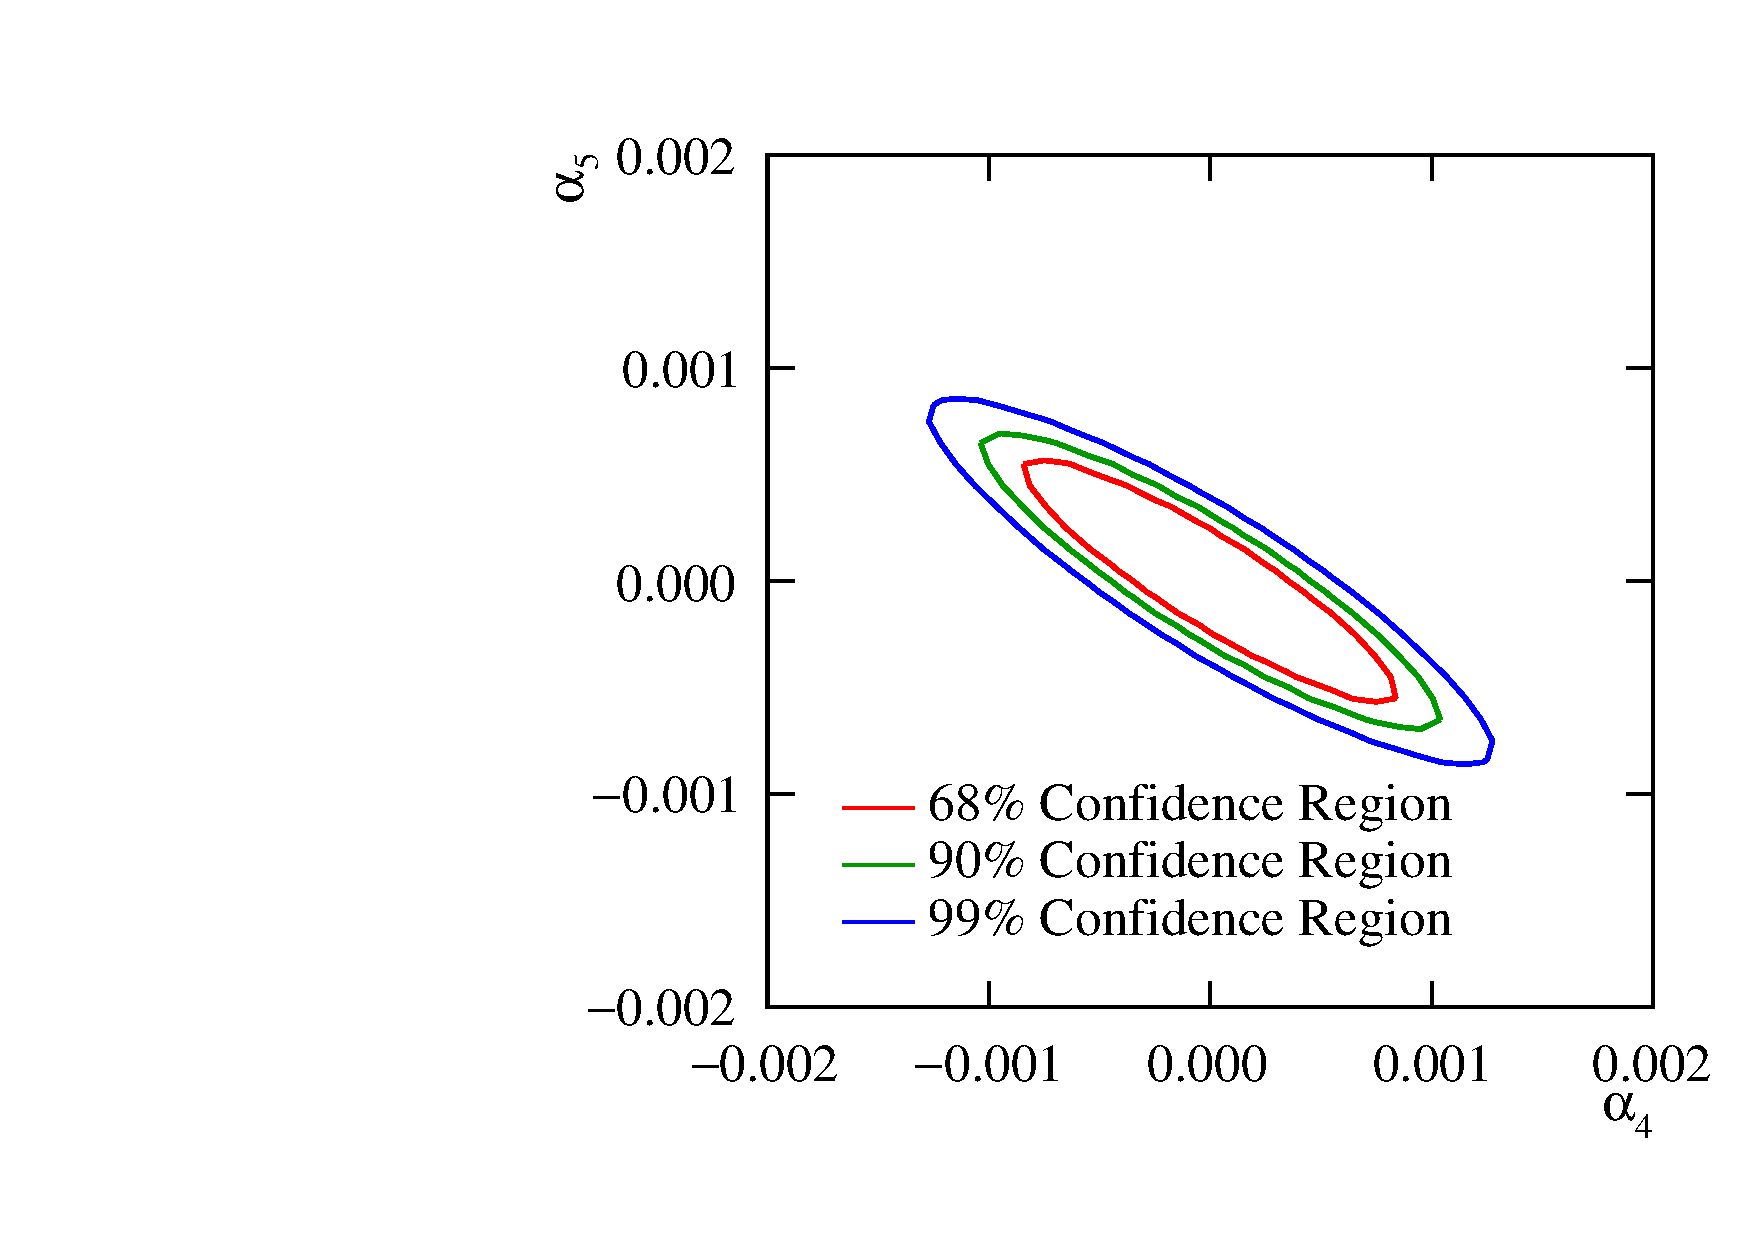
\includegraphics[width=0.3\textwidth]{PhysicsAnalysis/Plots/Chi2ContoursOptimisation/3000GeV/KtSPFOsR1p10.pdf}}\hfill
\subfloat[][Longitudinally Invariant Kt Algorithm, R = 0.7, Tight Selected PFOs, 3 TeV Events]{\label{fig:chi2jetalgoptkt0p70tpfos3000GeV} 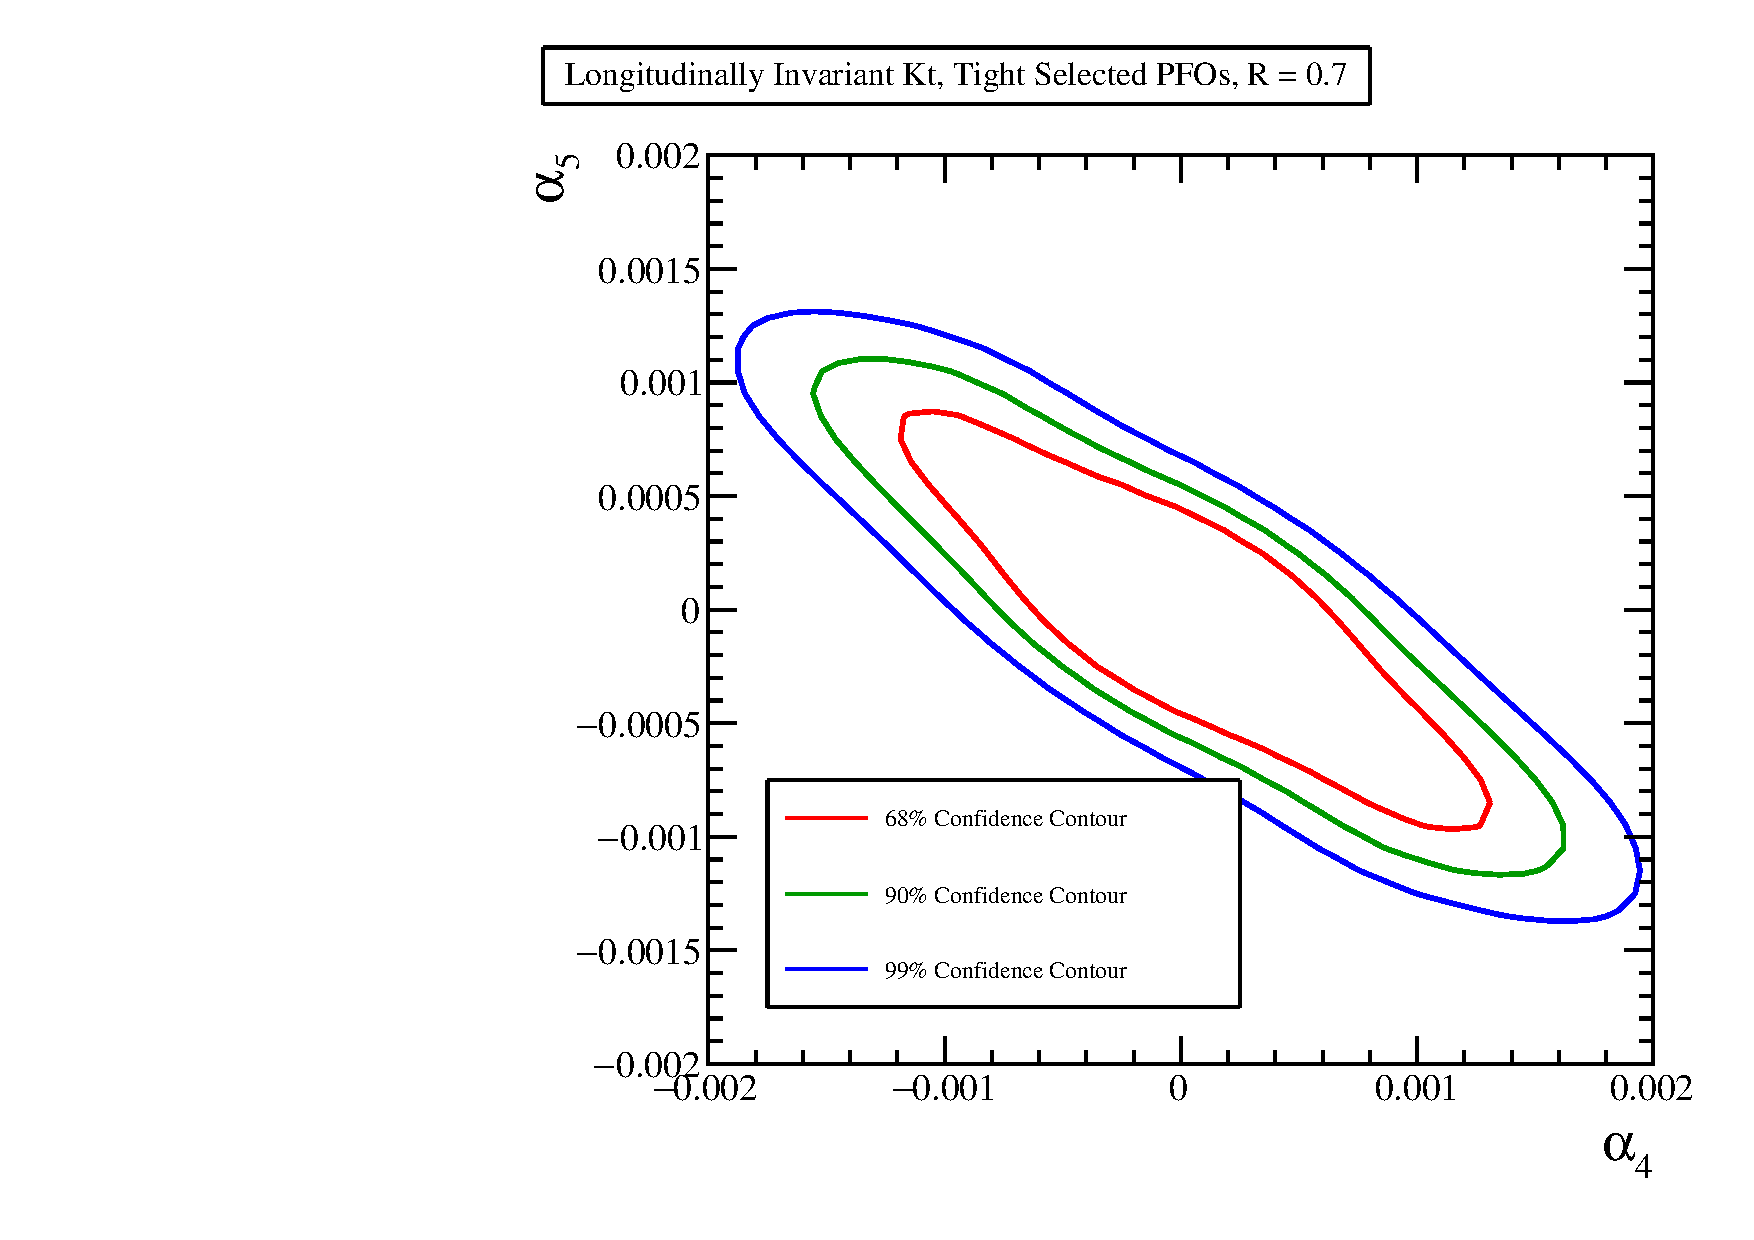
\includegraphics[width=0.3\textwidth]{PhysicsAnalysis/Plots/Chi2ContoursOptimisation/3000GeV/KtTPFOsR0p70.pdf}}
\subfloat[][Longitudinally Invariant Kt Algorithm, R = 0.9, Tight Selected PFOs, 3 TeV Events]{\label{fig:chi2jetalgoptkt0p90tpfos3000GeV} 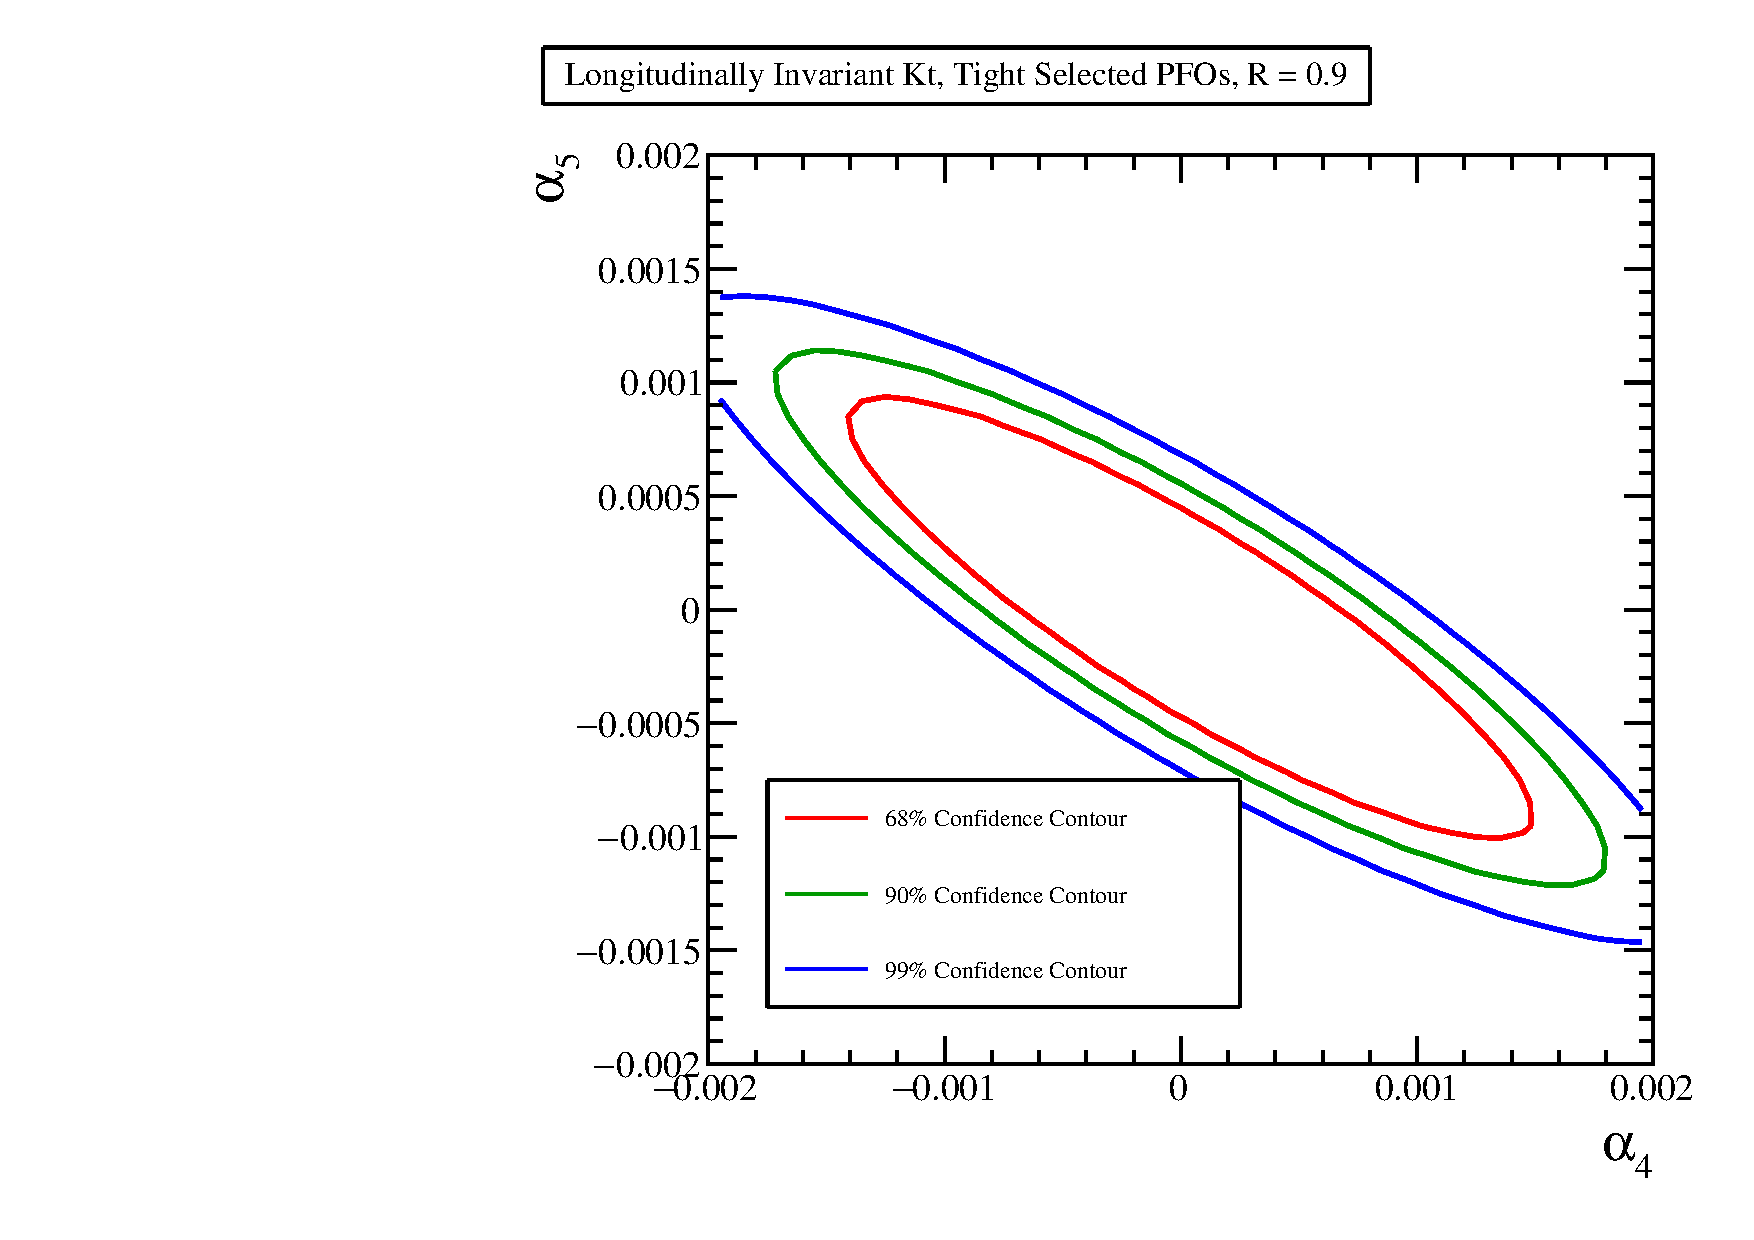
\includegraphics[width=0.3\textwidth]{PhysicsAnalysis/Plots/Chi2ContoursOptimisation/3000GeV/KtTPFOsR0p90.pdf}}
\subfloat[][Longitudinally Invariant Kt Algorithm, R = 1.1, Tight Selected PFOs, 3 TeV Events]{\label{fig:chi2jetalgoptkt1p10tpfos3000GeV} 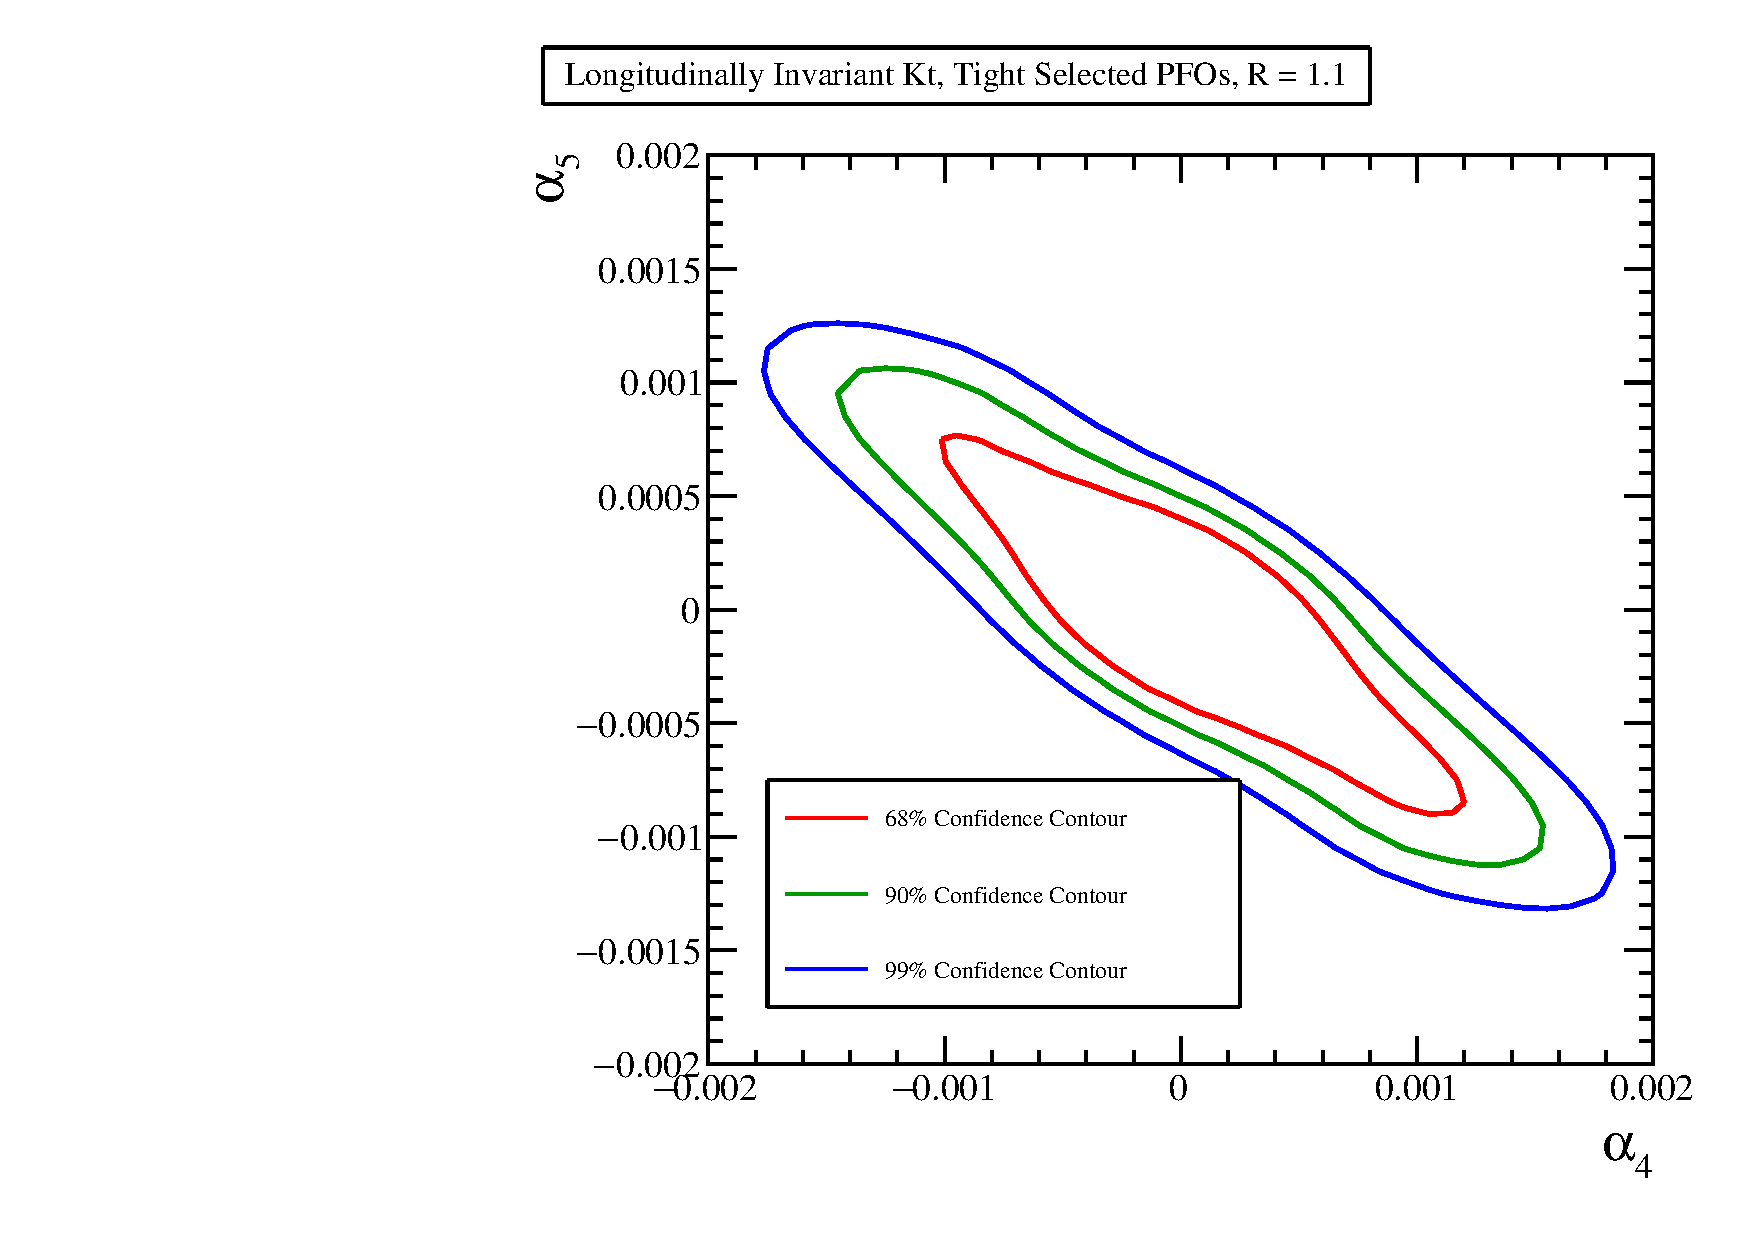
\includegraphics[width=0.3\textwidth]{PhysicsAnalysis/Plots/Chi2ContoursOptimisation/3000GeV/KtTPFOsR1p10.pdf}}\hfill
\caption[$\chi^{2}$ Sensitivity contours for the $\text{qqqq}\nu\nu$ final state arising from a fit to $\text{cos}\theta^{*}_{\text{Jets}}$ at 1.4 TeV for different values of jet reconstruction parameters.]{$\chi^{2}$ Sensitivity contours for the $\text{qqqq}\nu\nu$ final state arising from a fit to $\text{cos}\theta^{*}_{\text{Jets}}$ at 1.4 TeV for different values of jet reconstruction parameters.}
\label{fig:chi2jetalgopt1400GeV}
\end{figure}


%% Big appendixes should be split off into separate files, just like chapters
%\input{app-myreallybigappendix}
